% Options for packages loaded elsewhere
\PassOptionsToPackage{unicode}{hyperref}
\PassOptionsToPackage{hyphens}{url}
%
\documentclass[
]{article}
\usepackage{amsmath,amssymb}
\usepackage{iftex}
\ifPDFTeX
  \usepackage[T1]{fontenc}
  \usepackage[utf8]{inputenc}
  \usepackage{textcomp} % provide euro and other symbols
\else % if luatex or xetex
  \usepackage{unicode-math} % this also loads fontspec
  \defaultfontfeatures{Scale=MatchLowercase}
  \defaultfontfeatures[\rmfamily]{Ligatures=TeX,Scale=1}
\fi
\usepackage{lmodern}
\ifPDFTeX\else
  % xetex/luatex font selection
\fi
% Use upquote if available, for straight quotes in verbatim environments
\IfFileExists{upquote.sty}{\usepackage{upquote}}{}
\IfFileExists{microtype.sty}{% use microtype if available
  \usepackage[]{microtype}
  \UseMicrotypeSet[protrusion]{basicmath} % disable protrusion for tt fonts
}{}
\makeatletter
\@ifundefined{KOMAClassName}{% if non-KOMA class
  \IfFileExists{parskip.sty}{%
    \usepackage{parskip}
  }{% else
    \setlength{\parindent}{0pt}
    \setlength{\parskip}{6pt plus 2pt minus 1pt}}
}{% if KOMA class
  \KOMAoptions{parskip=half}}
\makeatother
\usepackage{xcolor}
\usepackage[margin=1in]{geometry}
\usepackage{color}
\usepackage{fancyvrb}
\newcommand{\VerbBar}{|}
\newcommand{\VERB}{\Verb[commandchars=\\\{\}]}
\DefineVerbatimEnvironment{Highlighting}{Verbatim}{commandchars=\\\{\}}
% Add ',fontsize=\small' for more characters per line
\usepackage{framed}
\definecolor{shadecolor}{RGB}{248,248,248}
\newenvironment{Shaded}{\begin{snugshade}}{\end{snugshade}}
\newcommand{\AlertTok}[1]{\textcolor[rgb]{0.94,0.16,0.16}{#1}}
\newcommand{\AnnotationTok}[1]{\textcolor[rgb]{0.56,0.35,0.01}{\textbf{\textit{#1}}}}
\newcommand{\AttributeTok}[1]{\textcolor[rgb]{0.13,0.29,0.53}{#1}}
\newcommand{\BaseNTok}[1]{\textcolor[rgb]{0.00,0.00,0.81}{#1}}
\newcommand{\BuiltInTok}[1]{#1}
\newcommand{\CharTok}[1]{\textcolor[rgb]{0.31,0.60,0.02}{#1}}
\newcommand{\CommentTok}[1]{\textcolor[rgb]{0.56,0.35,0.01}{\textit{#1}}}
\newcommand{\CommentVarTok}[1]{\textcolor[rgb]{0.56,0.35,0.01}{\textbf{\textit{#1}}}}
\newcommand{\ConstantTok}[1]{\textcolor[rgb]{0.56,0.35,0.01}{#1}}
\newcommand{\ControlFlowTok}[1]{\textcolor[rgb]{0.13,0.29,0.53}{\textbf{#1}}}
\newcommand{\DataTypeTok}[1]{\textcolor[rgb]{0.13,0.29,0.53}{#1}}
\newcommand{\DecValTok}[1]{\textcolor[rgb]{0.00,0.00,0.81}{#1}}
\newcommand{\DocumentationTok}[1]{\textcolor[rgb]{0.56,0.35,0.01}{\textbf{\textit{#1}}}}
\newcommand{\ErrorTok}[1]{\textcolor[rgb]{0.64,0.00,0.00}{\textbf{#1}}}
\newcommand{\ExtensionTok}[1]{#1}
\newcommand{\FloatTok}[1]{\textcolor[rgb]{0.00,0.00,0.81}{#1}}
\newcommand{\FunctionTok}[1]{\textcolor[rgb]{0.13,0.29,0.53}{\textbf{#1}}}
\newcommand{\ImportTok}[1]{#1}
\newcommand{\InformationTok}[1]{\textcolor[rgb]{0.56,0.35,0.01}{\textbf{\textit{#1}}}}
\newcommand{\KeywordTok}[1]{\textcolor[rgb]{0.13,0.29,0.53}{\textbf{#1}}}
\newcommand{\NormalTok}[1]{#1}
\newcommand{\OperatorTok}[1]{\textcolor[rgb]{0.81,0.36,0.00}{\textbf{#1}}}
\newcommand{\OtherTok}[1]{\textcolor[rgb]{0.56,0.35,0.01}{#1}}
\newcommand{\PreprocessorTok}[1]{\textcolor[rgb]{0.56,0.35,0.01}{\textit{#1}}}
\newcommand{\RegionMarkerTok}[1]{#1}
\newcommand{\SpecialCharTok}[1]{\textcolor[rgb]{0.81,0.36,0.00}{\textbf{#1}}}
\newcommand{\SpecialStringTok}[1]{\textcolor[rgb]{0.31,0.60,0.02}{#1}}
\newcommand{\StringTok}[1]{\textcolor[rgb]{0.31,0.60,0.02}{#1}}
\newcommand{\VariableTok}[1]{\textcolor[rgb]{0.00,0.00,0.00}{#1}}
\newcommand{\VerbatimStringTok}[1]{\textcolor[rgb]{0.31,0.60,0.02}{#1}}
\newcommand{\WarningTok}[1]{\textcolor[rgb]{0.56,0.35,0.01}{\textbf{\textit{#1}}}}
\usepackage{graphicx}
\makeatletter
\def\maxwidth{\ifdim\Gin@nat@width>\linewidth\linewidth\else\Gin@nat@width\fi}
\def\maxheight{\ifdim\Gin@nat@height>\textheight\textheight\else\Gin@nat@height\fi}
\makeatother
% Scale images if necessary, so that they will not overflow the page
% margins by default, and it is still possible to overwrite the defaults
% using explicit options in \includegraphics[width, height, ...]{}
\setkeys{Gin}{width=\maxwidth,height=\maxheight,keepaspectratio}
% Set default figure placement to htbp
\makeatletter
\def\fps@figure{htbp}
\makeatother
\setlength{\emergencystretch}{3em} % prevent overfull lines
\providecommand{\tightlist}{%
  \setlength{\itemsep}{0pt}\setlength{\parskip}{0pt}}
\setcounter{secnumdepth}{-\maxdimen} % remove section numbering
\usepackage{fvextra}
\DefineVerbatimEnvironment{Highlighting}{Verbatim}{
breaklines=true,
commandchars=\\\{\},
fontsize=\normalsize
}
\ifLuaTeX
  \usepackage{selnolig}  % disable illegal ligatures
\fi
\usepackage{bookmark}
\IfFileExists{xurl.sty}{\usepackage{xurl}}{} % add URL line breaks if available
\urlstyle{same}
\hypersetup{
  pdftitle={Saltmarsh Habitat Classification Models},
  pdfauthor={Alyssa Bueno},
  hidelinks,
  pdfcreator={LaTeX via pandoc}}

\title{Saltmarsh Habitat Classification Models}
\author{Alyssa Bueno}
\date{2025-08-02}

\begin{document}
\maketitle

\subsection{Saltmarsh Habitat
Classification}\label{saltmarsh-habitat-classification}

This code outlines 4 different model classification iterations, each
differing by the input layers.

\begin{enumerate}
\def\labelenumi{\arabic{enumi}.}
\tightlist
\item
  NDWI + NDVI + PCA + NAIP + Brightness
\item
  NDWI + NDVI + PCA
\item
  NAIP + NDVI
\item
  PCA
\end{enumerate}

\section{Setup: Ingest the training data and set up the
layers}\label{setup-ingest-the-training-data-and-set-up-the-layers}

\begin{Shaded}
\begin{Highlighting}[]
\CommentTok{\# load raster and training polygons}
\NormalTok{naip }\OtherTok{\textless{}{-}} \FunctionTok{rast}\NormalTok{(}\StringTok{"training\_raster\_round\_5.tif"}\NormalTok{) }\CommentTok{\# this has the raster data    }
\NormalTok{training\_polygons }\OtherTok{\textless{}{-}} \FunctionTok{vect}\NormalTok{(}\StringTok{"training\_polygons\_round\_5.shp"}\NormalTok{) }\CommentTok{\# this has the classes}

\FunctionTok{names}\NormalTok{(naip) }\OtherTok{\textless{}{-}} \FunctionTok{paste0}\NormalTok{(}\StringTok{"naip"}\NormalTok{, }\DecValTok{1}\SpecialCharTok{:}\DecValTok{4}\NormalTok{) }\CommentTok{\# change name of naip bands layer}

\CommentTok{\# calculate NDVI}
\NormalTok{ndvi }\OtherTok{\textless{}{-}}\NormalTok{ (naip[[}\DecValTok{4}\NormalTok{]] }\SpecialCharTok{{-}}\NormalTok{ naip[[}\DecValTok{1}\NormalTok{]]) }\SpecialCharTok{/}\NormalTok{ (naip[[}\DecValTok{4}\NormalTok{]] }\SpecialCharTok{+}\NormalTok{ naip[[}\DecValTok{1}\NormalTok{]])}
\FunctionTok{names}\NormalTok{(ndvi) }\OtherTok{\textless{}{-}} \StringTok{"ndvi"}

\CommentTok{\# calculate brightness}
\NormalTok{brightness }\OtherTok{\textless{}{-}}\NormalTok{ (naip[[}\DecValTok{1}\NormalTok{]] }\SpecialCharTok{+}\NormalTok{ naip[[}\DecValTok{2}\NormalTok{]] }\SpecialCharTok{+}\NormalTok{ naip[[}\DecValTok{3}\NormalTok{]] }\SpecialCharTok{+}\NormalTok{ naip[[}\DecValTok{4}\NormalTok{]]) }\SpecialCharTok{/} \DecValTok{4}
\FunctionTok{names}\NormalTok{(brightness) }\OtherTok{\textless{}{-}} \StringTok{"brightness"}

\CommentTok{\# calculate ndwi}
\NormalTok{ndwi }\OtherTok{\textless{}{-}}\NormalTok{ (naip[[}\DecValTok{4}\NormalTok{]] }\SpecialCharTok{{-}}\NormalTok{ naip[[}\DecValTok{2}\NormalTok{]]) }\SpecialCharTok{/}\NormalTok{ (naip[[}\DecValTok{4}\NormalTok{]] }\SpecialCharTok{+}\NormalTok{ naip[[}\DecValTok{2}\NormalTok{]])}
\FunctionTok{names}\NormalTok{(ndwi) }\OtherTok{\textless{}{-}} \StringTok{"ndwi"}

\CommentTok{\# now create the PCA }

\NormalTok{all\_for\_pca }\OtherTok{\textless{}{-}} \FunctionTok{c}\NormalTok{(naip, ndvi)  }\CommentTok{\# add ndvi to the raster}
\NormalTok{vals }\OtherTok{\textless{}{-}} \FunctionTok{values}\NormalTok{(all\_for\_pca)}
\NormalTok{vals }\OtherTok{\textless{}{-}}\NormalTok{ vals[}\FunctionTok{complete.cases}\NormalTok{(vals), ]}
\NormalTok{pca\_pixels }\OtherTok{\textless{}{-}} \FunctionTok{prcomp}\NormalTok{(vals, }\AttributeTok{center =} \ConstantTok{TRUE}\NormalTok{, }\AttributeTok{scale. =} \ConstantTok{TRUE}\NormalTok{)}
\NormalTok{pca }\OtherTok{\textless{}{-}} \FunctionTok{predict}\NormalTok{(all\_for\_pca, pca\_pixels, }\AttributeTok{index =} \DecValTok{1}\SpecialCharTok{:}\DecValTok{5}\NormalTok{)  }\CommentTok{\# for 5 PCs}
\end{Highlighting}
\end{Shaded}

\begin{verbatim}
## |---------|---------|---------|---------|=========================================                                          
\end{verbatim}

\begin{Shaded}
\begin{Highlighting}[]
\FunctionTok{names}\NormalTok{(pca) }\OtherTok{\textless{}{-}} \FunctionTok{paste0}\NormalTok{(}\StringTok{"PCA"}\NormalTok{, }\DecValTok{1}\SpecialCharTok{:}\DecValTok{5}\NormalTok{)}
\end{Highlighting}
\end{Shaded}

\section{1. First Iteration: NDWI + NDVI + PCA + NAIP +
Brightness}\label{first-iteration-ndwi-ndvi-pca-naip-brightness}

\begin{Shaded}
\begin{Highlighting}[]
\CommentTok{\# stack em up}
\NormalTok{r\_stack }\OtherTok{\textless{}{-}} \FunctionTok{c}\NormalTok{(ndwi, ndvi, pca, naip, brightness)}

\CommentTok{\# extract raster values for training polygons}
\NormalTok{extracted }\OtherTok{\textless{}{-}}\NormalTok{ terra}\SpecialCharTok{::}\FunctionTok{extract}\NormalTok{(r\_stack, training\_polygons, }\AttributeTok{df =} \ConstantTok{TRUE}\NormalTok{)}

\CommentTok{\# turn class into a factor}
\NormalTok{training\_polygons}\SpecialCharTok{$}\NormalTok{class }\OtherTok{\textless{}{-}} \FunctionTok{as.factor}\NormalTok{(training\_polygons}\SpecialCharTok{$}\NormalTok{class)}

\CommentTok{\# Convert training\_polygons to dataframe to get the class labels}
\NormalTok{poly\_df }\OtherTok{\textless{}{-}} \FunctionTok{as.data.frame}\NormalTok{(training\_polygons)}
\NormalTok{poly\_df}\SpecialCharTok{$}\NormalTok{ID }\OtherTok{\textless{}{-}} \DecValTok{1}\SpecialCharTok{:}\FunctionTok{nrow}\NormalTok{(poly\_df)  }\CommentTok{\# Add ID column to match extract output}

\CommentTok{\# Join the class labels}
\NormalTok{extracted }\OtherTok{\textless{}{-}}\NormalTok{ extracted }\SpecialCharTok{\%\textgreater{}\%}
  \FunctionTok{left\_join}\NormalTok{(poly\_df[, }\FunctionTok{c}\NormalTok{(}\StringTok{"ID"}\NormalTok{, }\StringTok{"class"}\NormalTok{)], }\AttributeTok{by =} \StringTok{"ID"}\NormalTok{)}

\CommentTok{\# clean data by removing rows with na values and remove ID column}
\NormalTok{extracted\_clean }\OtherTok{\textless{}{-}} \FunctionTok{na.omit}\NormalTok{(extracted[, }\SpecialCharTok{{-}}\DecValTok{1}\NormalTok{])  }\CommentTok{\# remove ID and NAs}

\CommentTok{\# sample 2000 per class}
\NormalTok{training\_data }\OtherTok{\textless{}{-}}\NormalTok{ extracted\_clean }\SpecialCharTok{\%\textgreater{}\%}
  \FunctionTok{group\_by}\NormalTok{(class) }\SpecialCharTok{\%\textgreater{}\%}
  \FunctionTok{sample\_n}\NormalTok{(}\FunctionTok{min}\NormalTok{(}\DecValTok{2000}\NormalTok{, }\FunctionTok{n}\NormalTok{())) }\SpecialCharTok{\%\textgreater{}\%}  \CommentTok{\# Use min() to handle small classes}
  \FunctionTok{ungroup}\NormalTok{()}

\CommentTok{\# turn class column into factor}
\NormalTok{training\_data}\SpecialCharTok{$}\NormalTok{class }\OtherTok{\textless{}{-}} \FunctionTok{factor}\NormalTok{(training\_data}\SpecialCharTok{$}\NormalTok{class)}

\CommentTok{\# check the sampling balance in the classes}
\FunctionTok{print}\NormalTok{(}\FunctionTok{table}\NormalTok{(training\_data}\SpecialCharTok{$}\NormalTok{class))}
\end{Highlighting}
\end{Shaded}

\begin{verbatim}
## 
##   hm   lm   md   ow   ph   rd   up 
## 2000 2000 2000 2000 2000 2000 2000
\end{verbatim}

\begin{Shaded}
\begin{Highlighting}[]
\CommentTok{\# split training and test data}
\FunctionTok{set.seed}\NormalTok{(}\DecValTok{342}\NormalTok{)}
\NormalTok{idx }\OtherTok{\textless{}{-}} \FunctionTok{sample}\NormalTok{(}\FunctionTok{seq\_len}\NormalTok{(}\FunctionTok{nrow}\NormalTok{(training\_data)), }\AttributeTok{size =} \FloatTok{0.8} \SpecialCharTok{*} \FunctionTok{nrow}\NormalTok{(training\_data))}
\NormalTok{train\_set }\OtherTok{\textless{}{-}}\NormalTok{ training\_data[idx, ]}
\NormalTok{test\_set  }\OtherTok{\textless{}{-}}\NormalTok{ training\_data[}\SpecialCharTok{{-}}\NormalTok{idx, ]}

\CommentTok{\# train random forest model}
\NormalTok{rf\_model }\OtherTok{\textless{}{-}} \FunctionTok{randomForest}\NormalTok{(class }\SpecialCharTok{\textasciitilde{}}\NormalTok{ ., }
                         \AttributeTok{data =}\NormalTok{ train\_set, }
                         \AttributeTok{ntree =} \DecValTok{500}\NormalTok{)}

\CommentTok{\# validation metrics}
\NormalTok{preds }\OtherTok{\textless{}{-}} \FunctionTok{predict}\NormalTok{(rf\_model, }\AttributeTok{newdata =}\NormalTok{ test\_set)}
\NormalTok{accuracy }\OtherTok{\textless{}{-}} \FunctionTok{mean}\NormalTok{(preds }\SpecialCharTok{==}\NormalTok{ test\_set}\SpecialCharTok{$}\NormalTok{class)}
\FunctionTok{cat}\NormalTok{(}\StringTok{"Accuracy:"}\NormalTok{, }\FunctionTok{round}\NormalTok{(accuracy, }\DecValTok{4}\NormalTok{), }\StringTok{"}\SpecialCharTok{\textbackslash{}n}\StringTok{"}\NormalTok{)}
\end{Highlighting}
\end{Shaded}

\begin{verbatim}
## Accuracy: 0.9832
\end{verbatim}

\begin{Shaded}
\begin{Highlighting}[]
\FunctionTok{print}\NormalTok{(rf\_model)}
\end{Highlighting}
\end{Shaded}

\begin{verbatim}
## 
## Call:
##  randomForest(formula = class ~ ., data = train_set, ntree = 500) 
##                Type of random forest: classification
##                      Number of trees: 500
## No. of variables tried at each split: 3
## 
##         OOB estimate of  error rate: 1.88%
## Confusion matrix:
##      hm   lm   md   ow   ph   rd   up class.error
## hm 1595   10    0    0    0    2    0 0.007467330
## lm   13 1550    1    0   30    1    2 0.029430182
## md    0    0 1594    0    0    7    0 0.004372267
## ow    0    0    0 1589    0    0    0 0.000000000
## ph    0   42    0    0 1552    3   15 0.037220844
## rd    9    4   19    0   11 1562    0 0.026791277
## up    1   18    0    0   22    1 1547 0.026431718
\end{verbatim}

\begin{Shaded}
\begin{Highlighting}[]
\CommentTok{\# confusion matrix}
\FunctionTok{confusionMatrix}\NormalTok{(preds, test\_set}\SpecialCharTok{$}\NormalTok{class)}
\end{Highlighting}
\end{Shaded}

\begin{verbatim}
## Confusion Matrix and Statistics
## 
##           Reference
## Prediction  hm  lm  md  ow  ph  rd  up
##         hm 387   4   0   0   0   1   4
##         lm   5 394   0   0  10   0   6
##         md   0   0 398   0   0   3   0
##         ow   0   0   0 411   0   0   0
##         ph   0   4   0   0 377   3   3
##         rd   1   0   1   0   0 388   0
##         up   0   1   0   0   1   0 398
## 
## Overall Statistics
##                                           
##                Accuracy : 0.9832          
##                  95% CI : (0.9777, 0.9876)
##     No Information Rate : 0.1468          
##     P-Value [Acc > NIR] : < 2.2e-16       
##                                           
##                   Kappa : 0.9804          
##                                           
##  Mcnemar's Test P-Value : NA              
## 
## Statistics by Class:
## 
##                      Class: hm Class: lm Class: md Class: ow Class: ph
## Sensitivity             0.9847    0.9777    0.9975    1.0000    0.9716
## Specificity             0.9963    0.9912    0.9988    1.0000    0.9959
## Pos Pred Value          0.9773    0.9494    0.9925    1.0000    0.9742
## Neg Pred Value          0.9975    0.9962    0.9996    1.0000    0.9954
## Prevalence              0.1404    0.1439    0.1425    0.1468    0.1386
## Detection Rate          0.1382    0.1407    0.1421    0.1468    0.1346
## Detection Prevalence    0.1414    0.1482    0.1432    0.1468    0.1382
## Balanced Accuracy       0.9905    0.9845    0.9981    1.0000    0.9838
##                      Class: rd Class: up
## Sensitivity             0.9823    0.9684
## Specificity             0.9992    0.9992
## Pos Pred Value          0.9949    0.9950
## Neg Pred Value          0.9971    0.9946
## Prevalence              0.1411    0.1468
## Detection Rate          0.1386    0.1421
## Detection Prevalence    0.1393    0.1429
## Balanced Accuracy       0.9907    0.9838
\end{verbatim}

\section{classifying the plots}\label{classifying-the-plots}

\begin{Shaded}
\begin{Highlighting}[]
\CommentTok{\# load the new, unlabeled raster}
\NormalTok{prediction\_raster }\OtherTok{\textless{}{-}} \FunctionTok{rast}\NormalTok{(}\StringTok{"\textasciitilde{}/Desktop/marshbirdsoutput/round\_5/prediction\_raster\_round\_5.tif"}\NormalTok{)}

\CommentTok{\# calculate NDVI for prediction raster}
\NormalTok{ndvi\_pred }\OtherTok{\textless{}{-}}\NormalTok{ (prediction\_raster[[}\DecValTok{4}\NormalTok{]] }\SpecialCharTok{{-}}\NormalTok{ prediction\_raster[[}\DecValTok{1}\NormalTok{]]) }\SpecialCharTok{/} 
\NormalTok{  (prediction\_raster[[}\DecValTok{4}\NormalTok{]] }\SpecialCharTok{+}\NormalTok{ prediction\_raster[[}\DecValTok{1}\NormalTok{]])}
\FunctionTok{names}\NormalTok{(ndvi\_pred) }\OtherTok{\textless{}{-}} \StringTok{"ndvi"}

\CommentTok{\# calculation NDWI}
\NormalTok{ndwi\_pred }\OtherTok{\textless{}{-}}\NormalTok{ (prediction\_raster[[}\DecValTok{4}\NormalTok{]] }\SpecialCharTok{{-}}\NormalTok{ prediction\_raster[[}\DecValTok{2}\NormalTok{]]) }\SpecialCharTok{/} 
\NormalTok{  (prediction\_raster[[}\DecValTok{4}\NormalTok{]] }\SpecialCharTok{+}\NormalTok{ prediction\_raster[[}\DecValTok{2}\NormalTok{]])}
\FunctionTok{names}\NormalTok{(ndwi\_pred) }\OtherTok{\textless{}{-}} \StringTok{"ndwi"}

\CommentTok{\# Calculate brightness}
\NormalTok{brightness\_pred }\OtherTok{\textless{}{-}}\NormalTok{ (prediction\_raster[[}\DecValTok{1}\NormalTok{]] }\SpecialCharTok{+}\NormalTok{ prediction\_raster[[}\DecValTok{2}\NormalTok{]] }\SpecialCharTok{+} 
\NormalTok{                      prediction\_raster[[}\DecValTok{3}\NormalTok{]] }\SpecialCharTok{+}\NormalTok{ prediction\_raster[[}\DecValTok{4}\NormalTok{]]) }\SpecialCharTok{/} \DecValTok{4}
\FunctionTok{names}\NormalTok{(brightness\_pred) }\OtherTok{\textless{}{-}} \StringTok{"brightness"}

\CommentTok{\# Apply the pca}
\NormalTok{all\_for\_pca\_pred }\OtherTok{\textless{}{-}} \FunctionTok{c}\NormalTok{(prediction\_raster, ndvi\_pred)}
\FunctionTok{names}\NormalTok{(all\_for\_pca\_pred) }\OtherTok{\textless{}{-}} \FunctionTok{names}\NormalTok{(all\_for\_pca)  }\CommentTok{\# ensure exact match}
\NormalTok{pca\_pred }\OtherTok{\textless{}{-}} \FunctionTok{predict}\NormalTok{(all\_for\_pca\_pred, pca\_pixels, }\AttributeTok{index =} \DecValTok{1}\SpecialCharTok{:}\DecValTok{5}\NormalTok{)}
\end{Highlighting}
\end{Shaded}

\begin{verbatim}
## |---------|---------|---------|---------|=========================================                                          
\end{verbatim}

\begin{Shaded}
\begin{Highlighting}[]
\FunctionTok{names}\NormalTok{(pca\_pred) }\OtherTok{\textless{}{-}} \FunctionTok{paste0}\NormalTok{(}\StringTok{"PCA"}\NormalTok{, }\DecValTok{1}\SpecialCharTok{:}\DecValTok{5}\NormalTok{)}

\CommentTok{\# stack it}
\NormalTok{prediction\_stack }\OtherTok{\textless{}{-}} \FunctionTok{c}\NormalTok{(prediction\_raster, ndvi\_pred, ndwi\_pred, brightness\_pred, pca\_pred)}

\CommentTok{\# rename to match training names}
\FunctionTok{names}\NormalTok{(prediction\_stack) }\OtherTok{\textless{}{-}} \FunctionTok{names}\NormalTok{(r\_stack)}

\CommentTok{\# apply the model to predict classes}
\NormalTok{classified }\OtherTok{\textless{}{-}} \FunctionTok{predict}\NormalTok{(prediction\_stack, rf\_model, }\AttributeTok{na.rm =} \ConstantTok{TRUE}\NormalTok{)}

\CommentTok{\# Define custom colors}
\NormalTok{colors }\OtherTok{\textless{}{-}} \FunctionTok{c}\NormalTok{(}
  \StringTok{"\#a6d96a"}\NormalTok{,  }\CommentTok{\# hm  }
  \StringTok{"\#1a9641"}\NormalTok{,  }\CommentTok{\# lm  }
  \StringTok{"\#8c510a"}\NormalTok{,  }\CommentTok{\# md  }
  \StringTok{"\#3288bd"}\NormalTok{,  }\CommentTok{\# ow  }
  \StringTok{"\#fdae61"}\NormalTok{,  }\CommentTok{\# ph  }
  \StringTok{"\#969696"}\NormalTok{,  }\CommentTok{\# rd  }
  \StringTok{"\#762a83"}   \CommentTok{\# up  }
\NormalTok{)}



\CommentTok{\# Plot with colors}
\FunctionTok{plot}\NormalTok{(classified, }\AttributeTok{col =}\NormalTok{ colors)}
\end{Highlighting}
\end{Shaded}

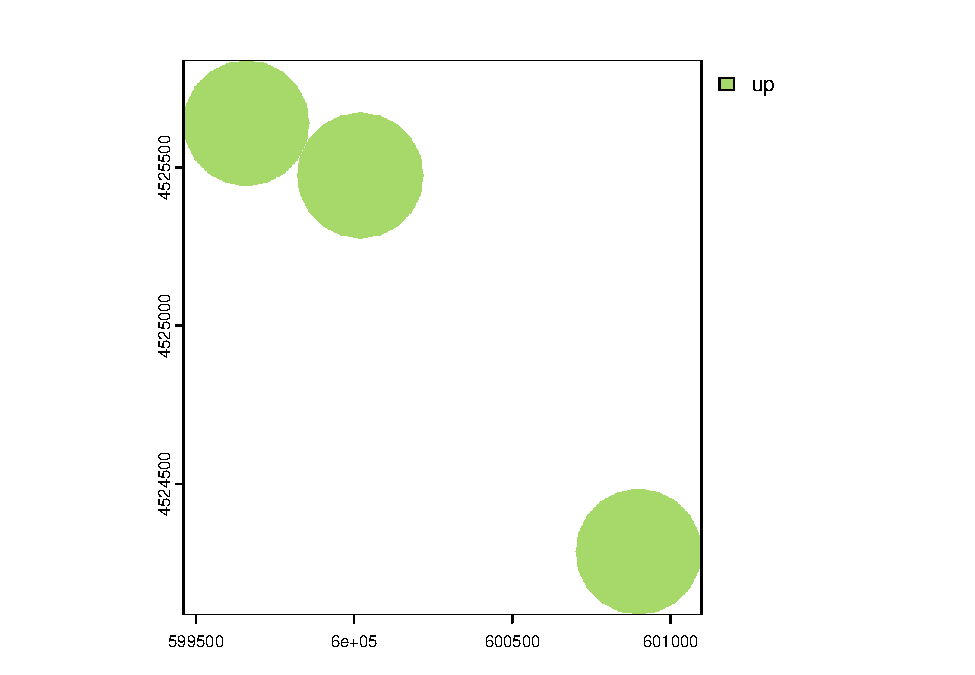
\includegraphics{veg_model_files/figure-latex/unnamed-chunk-4-1.pdf}

\begin{Shaded}
\begin{Highlighting}[]
\CommentTok{\# save the output tif}
\CommentTok{\# writeRaster(classified, "\textasciitilde{}/Desktop/marshbirdsoutput/round\_5/classified\_output.tif", overwrite = TRUE)}

\NormalTok{rf\_model}\SpecialCharTok{$}\NormalTok{importance}
\end{Highlighting}
\end{Shaded}

\begin{verbatim}
##            MeanDecreaseGini
## ndwi              1419.6837
## ndvi              1403.4559
## PCA1               774.4901
## PCA2               613.3142
## PCA3               585.1908
## PCA4               354.1295
## PCA5               404.8675
## naip1              571.6034
## naip2              539.3163
## naip3             1023.2475
## naip4             1089.1408
## brightness         820.6644
\end{verbatim}

\section{feature class importance and
visualizations}\label{feature-class-importance-and-visualizations}

\begin{Shaded}
\begin{Highlighting}[]
\FunctionTok{ggplot}\NormalTok{(training\_data, }\FunctionTok{aes}\NormalTok{(}\AttributeTok{x =}\NormalTok{ ndwi, }\AttributeTok{y =}\NormalTok{ ndvi, }\AttributeTok{color =}\NormalTok{ class)) }\SpecialCharTok{+}
  \FunctionTok{geom\_point}\NormalTok{(}\AttributeTok{alpha =} \FloatTok{0.3}\NormalTok{) }\SpecialCharTok{+}
  \FunctionTok{theme\_minimal}\NormalTok{()}
\end{Highlighting}
\end{Shaded}

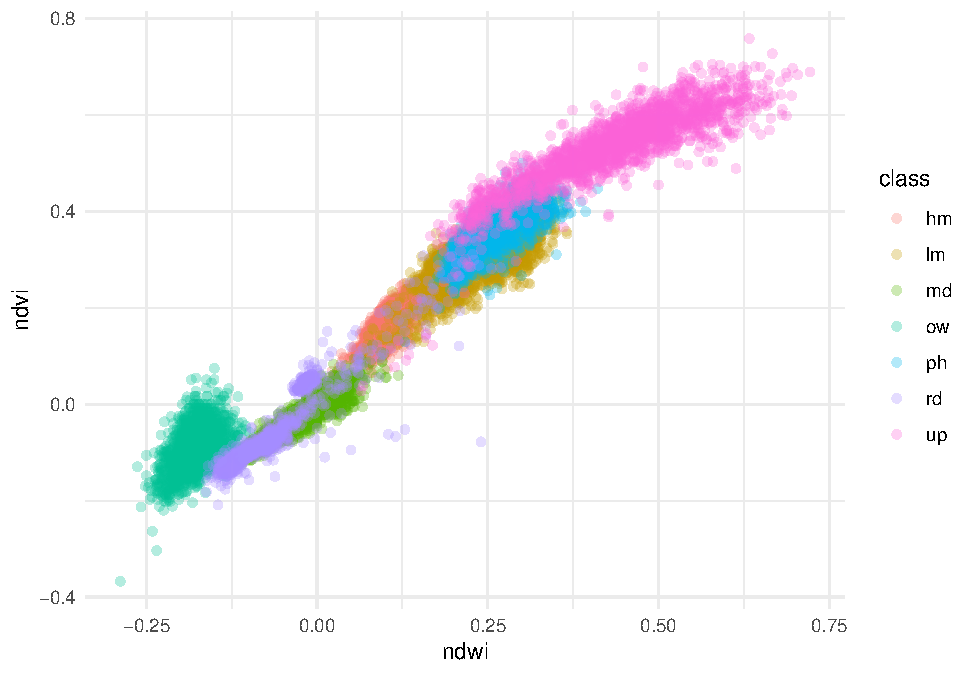
\includegraphics{veg_model_files/figure-latex/unnamed-chunk-5-1.pdf}

\begin{Shaded}
\begin{Highlighting}[]
\FunctionTok{ggplot}\NormalTok{(training\_data, }\FunctionTok{aes}\NormalTok{(}\AttributeTok{x =}\NormalTok{ ndwi, }\AttributeTok{fill =}\NormalTok{ class)) }\SpecialCharTok{+}
  \FunctionTok{geom\_density}\NormalTok{(}\AttributeTok{alpha =} \FloatTok{0.4}\NormalTok{, }\AttributeTok{color =} \ConstantTok{NA}\NormalTok{) }\SpecialCharTok{+}
  \FunctionTok{theme\_minimal}\NormalTok{()}
\end{Highlighting}
\end{Shaded}

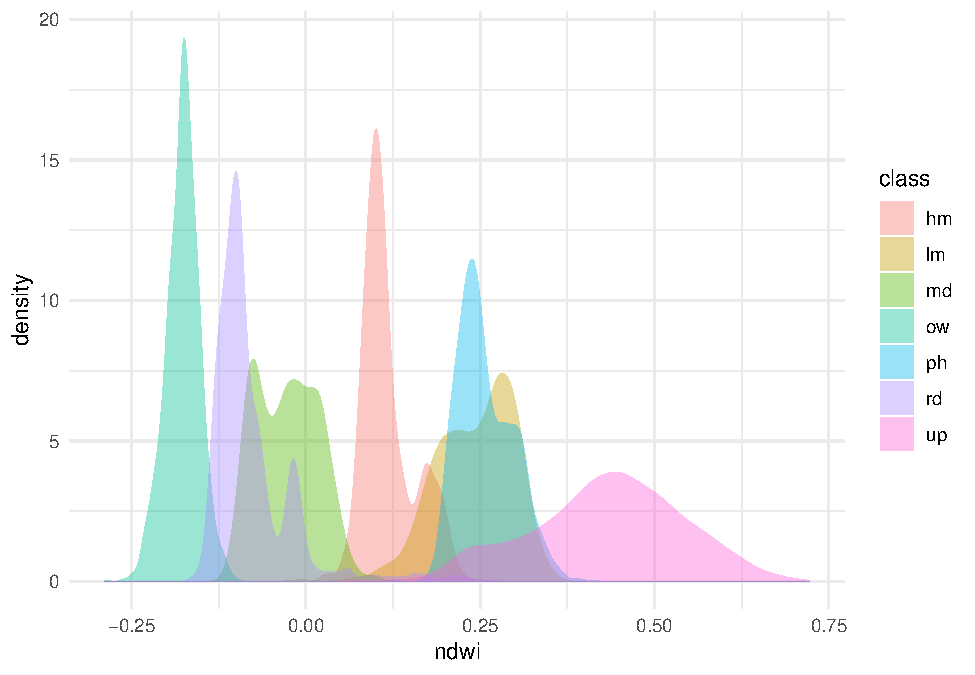
\includegraphics{veg_model_files/figure-latex/unnamed-chunk-5-2.pdf}

\begin{Shaded}
\begin{Highlighting}[]
\NormalTok{imp }\OtherTok{\textless{}{-}} \FunctionTok{as.data.frame}\NormalTok{(rf\_model}\SpecialCharTok{$}\NormalTok{importance)}
\NormalTok{imp}\SpecialCharTok{$}\NormalTok{feature }\OtherTok{\textless{}{-}} \FunctionTok{rownames}\NormalTok{(imp)}

\FunctionTok{ggplot}\NormalTok{(imp, }\FunctionTok{aes}\NormalTok{(}\AttributeTok{x =} \FunctionTok{reorder}\NormalTok{(feature, MeanDecreaseGini), }\AttributeTok{y =}\NormalTok{ MeanDecreaseGini)) }\SpecialCharTok{+}
  \FunctionTok{geom\_col}\NormalTok{(}\AttributeTok{fill =} \StringTok{"steelblue"}\NormalTok{) }\SpecialCharTok{+}
  \FunctionTok{coord\_flip}\NormalTok{() }\SpecialCharTok{+}
  \FunctionTok{labs}\NormalTok{(}\AttributeTok{title =} \StringTok{"Random Forest Variable Importance"}\NormalTok{,}
       \AttributeTok{x =} \StringTok{"Feature"}\NormalTok{, }\AttributeTok{y =} \StringTok{"Mean Decrease Gini"}\NormalTok{) }\SpecialCharTok{+}
  \FunctionTok{theme\_minimal}\NormalTok{()}
\end{Highlighting}
\end{Shaded}

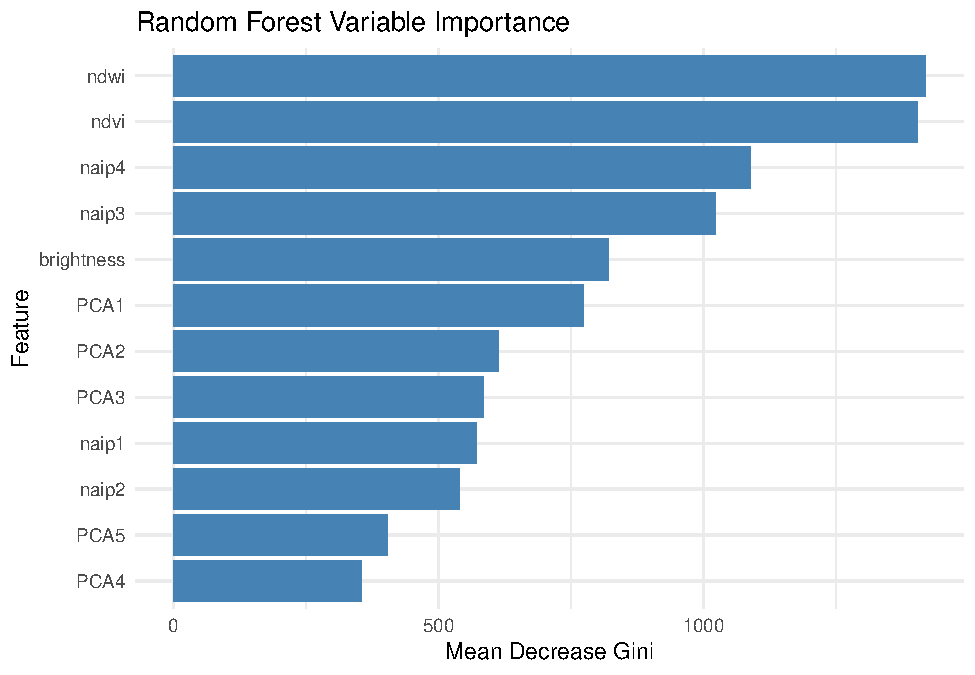
\includegraphics{veg_model_files/figure-latex/unnamed-chunk-5-3.pdf}

\section{2. Second Iteration: NAIP + NDVI +
NDWI}\label{second-iteration-naip-ndvi-ndwi}

\begin{Shaded}
\begin{Highlighting}[]
\CommentTok{\# stack em up}
\NormalTok{r\_stack }\OtherTok{\textless{}{-}} \FunctionTok{c}\NormalTok{(naip, ndvi, ndwi)}

\CommentTok{\# extract raster values for training polygons}
\NormalTok{extracted }\OtherTok{\textless{}{-}}\NormalTok{ terra}\SpecialCharTok{::}\FunctionTok{extract}\NormalTok{(r\_stack, training\_polygons, }\AttributeTok{df =} \ConstantTok{TRUE}\NormalTok{)}

\CommentTok{\# turn class into a factor}
\NormalTok{training\_polygons}\SpecialCharTok{$}\NormalTok{class }\OtherTok{\textless{}{-}} \FunctionTok{as.factor}\NormalTok{(training\_polygons}\SpecialCharTok{$}\NormalTok{class)}

\CommentTok{\# Convert training\_polygons to dataframe to get the class labels}
\NormalTok{poly\_df }\OtherTok{\textless{}{-}} \FunctionTok{as.data.frame}\NormalTok{(training\_polygons)}
\NormalTok{poly\_df}\SpecialCharTok{$}\NormalTok{ID }\OtherTok{\textless{}{-}} \DecValTok{1}\SpecialCharTok{:}\FunctionTok{nrow}\NormalTok{(poly\_df)  }\CommentTok{\# Add ID column to match extract output}

\CommentTok{\# Join the class labels}
\NormalTok{extracted }\OtherTok{\textless{}{-}}\NormalTok{ extracted }\SpecialCharTok{\%\textgreater{}\%}
  \FunctionTok{left\_join}\NormalTok{(poly\_df[, }\FunctionTok{c}\NormalTok{(}\StringTok{"ID"}\NormalTok{, }\StringTok{"class"}\NormalTok{)], }\AttributeTok{by =} \StringTok{"ID"}\NormalTok{)}

\CommentTok{\# clean data by removing rows with na values and remove ID column}
\NormalTok{extracted\_clean }\OtherTok{\textless{}{-}} \FunctionTok{na.omit}\NormalTok{(extracted[, }\SpecialCharTok{{-}}\DecValTok{1}\NormalTok{])  }\CommentTok{\# remove ID and NAs}

\CommentTok{\# sample 2000 per class}
\NormalTok{training\_data }\OtherTok{\textless{}{-}}\NormalTok{ extracted\_clean }\SpecialCharTok{\%\textgreater{}\%}
  \FunctionTok{group\_by}\NormalTok{(class) }\SpecialCharTok{\%\textgreater{}\%}
  \FunctionTok{sample\_n}\NormalTok{(}\FunctionTok{min}\NormalTok{(}\DecValTok{2000}\NormalTok{, }\FunctionTok{n}\NormalTok{())) }\SpecialCharTok{\%\textgreater{}\%}  \CommentTok{\# Use min() to handle small classes}
  \FunctionTok{ungroup}\NormalTok{()}

\CommentTok{\# turn class column into factor}
\NormalTok{training\_data}\SpecialCharTok{$}\NormalTok{class }\OtherTok{\textless{}{-}} \FunctionTok{factor}\NormalTok{(training\_data}\SpecialCharTok{$}\NormalTok{class)}
\end{Highlighting}
\end{Shaded}

\begin{Shaded}
\begin{Highlighting}[]
\CommentTok{\# split training and test data}
\FunctionTok{set.seed}\NormalTok{(}\DecValTok{342}\NormalTok{)}
\NormalTok{idx }\OtherTok{\textless{}{-}} \FunctionTok{sample}\NormalTok{(}\FunctionTok{seq\_len}\NormalTok{(}\FunctionTok{nrow}\NormalTok{(training\_data)), }\AttributeTok{size =} \FloatTok{0.8} \SpecialCharTok{*} \FunctionTok{nrow}\NormalTok{(training\_data))}
\NormalTok{train\_set }\OtherTok{\textless{}{-}}\NormalTok{ training\_data[idx, ]}
\NormalTok{test\_set  }\OtherTok{\textless{}{-}}\NormalTok{ training\_data[}\SpecialCharTok{{-}}\NormalTok{idx, ]}

\CommentTok{\# train random forest model}
\NormalTok{rf\_model }\OtherTok{\textless{}{-}} \FunctionTok{randomForest}\NormalTok{(class }\SpecialCharTok{\textasciitilde{}}\NormalTok{ ., }
                         \AttributeTok{data =}\NormalTok{ train\_set, }
                         \AttributeTok{ntree =} \DecValTok{500}\NormalTok{)}

\CommentTok{\# validation metrics}
\NormalTok{preds }\OtherTok{\textless{}{-}} \FunctionTok{predict}\NormalTok{(rf\_model, }\AttributeTok{newdata =}\NormalTok{ test\_set)}
\NormalTok{accuracy }\OtherTok{\textless{}{-}} \FunctionTok{mean}\NormalTok{(preds }\SpecialCharTok{==}\NormalTok{ test\_set}\SpecialCharTok{$}\NormalTok{class)}
\FunctionTok{cat}\NormalTok{(}\StringTok{"Accuracy:"}\NormalTok{, }\FunctionTok{round}\NormalTok{(accuracy, }\DecValTok{4}\NormalTok{), }\StringTok{"}\SpecialCharTok{\textbackslash{}n}\StringTok{"}\NormalTok{)}
\end{Highlighting}
\end{Shaded}

\begin{verbatim}
## Accuracy: 0.9814
\end{verbatim}

\begin{Shaded}
\begin{Highlighting}[]
\FunctionTok{print}\NormalTok{(rf\_model)}
\end{Highlighting}
\end{Shaded}

\begin{verbatim}
## 
## Call:
##  randomForest(formula = class ~ ., data = train_set, ntree = 500) 
##                Type of random forest: classification
##                      Number of trees: 500
## No. of variables tried at each split: 2
## 
##         OOB estimate of  error rate: 1.97%
## Confusion matrix:
##      hm   lm   md   ow   ph   rd   up  class.error
## hm 1596    8    0    0    1    2    0 0.0068450529
## lm   20 1544    1    0   29    0    3 0.0331872260
## md    0    1 1595    1    0    4    0 0.0037476577
## ow    0    0    0 1588    0    1    0 0.0006293266
## ph    0   45    0    0 1551    1   15 0.0378411911
## rd    7    2   13    0   10 1573    0 0.0199376947
## up    7   26    0    0   24    0 1532 0.0358716174
\end{verbatim}

\begin{Shaded}
\begin{Highlighting}[]
\CommentTok{\# confusion matrix}
\FunctionTok{confusionMatrix}\NormalTok{(preds, test\_set}\SpecialCharTok{$}\NormalTok{class)}
\end{Highlighting}
\end{Shaded}

\begin{verbatim}
## Confusion Matrix and Statistics
## 
##           Reference
## Prediction  hm  lm  md  ow  ph  rd  up
##         hm 389   4   0   0   0   1   1
##         lm   4 390   0   0  10   2   4
##         md   0   0 398   0   0   3   0
##         ow   0   0   0 411   0   0   0
##         ph   0   9   0   0 374   2   5
##         rd   0   0   1   0   0 386   1
##         up   0   0   0   0   4   1 400
## 
## Overall Statistics
##                                           
##                Accuracy : 0.9814          
##                  95% CI : (0.9757, 0.9861)
##     No Information Rate : 0.1468          
##     P-Value [Acc > NIR] : < 2.2e-16       
##                                           
##                   Kappa : 0.9783          
##                                           
##  Mcnemar's Test P-Value : NA              
## 
## Statistics by Class:
## 
##                      Class: hm Class: lm Class: md Class: ow Class: ph
## Sensitivity             0.9898    0.9677    0.9975    1.0000    0.9639
## Specificity             0.9975    0.9917    0.9988    1.0000    0.9934
## Pos Pred Value          0.9848    0.9512    0.9925    1.0000    0.9590
## Neg Pred Value          0.9983    0.9946    0.9996    1.0000    0.9942
## Prevalence              0.1404    0.1439    0.1425    0.1468    0.1386
## Detection Rate          0.1389    0.1393    0.1421    0.1468    0.1336
## Detection Prevalence    0.1411    0.1464    0.1432    0.1468    0.1393
## Balanced Accuracy       0.9937    0.9797    0.9981    1.0000    0.9786
##                      Class: rd Class: up
## Sensitivity             0.9772    0.9732
## Specificity             0.9992    0.9979
## Pos Pred Value          0.9948    0.9877
## Neg Pred Value          0.9963    0.9954
## Prevalence              0.1411    0.1468
## Detection Rate          0.1379    0.1429
## Detection Prevalence    0.1386    0.1446
## Balanced Accuracy       0.9882    0.9856
\end{verbatim}

\section{classifying the plots}\label{classifying-the-plots-1}

\begin{Shaded}
\begin{Highlighting}[]
\CommentTok{\# load the new, unlabeled raster}
\NormalTok{prediction\_raster }\OtherTok{\textless{}{-}} \FunctionTok{rast}\NormalTok{(}\StringTok{"\textasciitilde{}/Desktop/marshbirdsoutput/round\_5/prediction\_raster\_round\_5.tif"}\NormalTok{)}

\CommentTok{\# calculate NDVI for prediction raster}
\NormalTok{ndvi\_pred }\OtherTok{\textless{}{-}}\NormalTok{ (prediction\_raster[[}\DecValTok{4}\NormalTok{]] }\SpecialCharTok{{-}}\NormalTok{ prediction\_raster[[}\DecValTok{1}\NormalTok{]]) }\SpecialCharTok{/} 
\NormalTok{  (prediction\_raster[[}\DecValTok{4}\NormalTok{]] }\SpecialCharTok{+}\NormalTok{ prediction\_raster[[}\DecValTok{1}\NormalTok{]])}
\FunctionTok{names}\NormalTok{(ndvi\_pred) }\OtherTok{\textless{}{-}} \StringTok{"ndvi"}

\CommentTok{\# calculation NDWI}
\NormalTok{ndwi\_pred }\OtherTok{\textless{}{-}}\NormalTok{ (prediction\_raster[[}\DecValTok{4}\NormalTok{]] }\SpecialCharTok{{-}}\NormalTok{ prediction\_raster[[}\DecValTok{2}\NormalTok{]]) }\SpecialCharTok{/} 
\NormalTok{  (prediction\_raster[[}\DecValTok{4}\NormalTok{]] }\SpecialCharTok{+}\NormalTok{ prediction\_raster[[}\DecValTok{2}\NormalTok{]])}
\FunctionTok{names}\NormalTok{(ndwi\_pred) }\OtherTok{\textless{}{-}} \StringTok{"ndwi"}

\CommentTok{\# Calculate brightness}
\NormalTok{brightness\_pred }\OtherTok{\textless{}{-}}\NormalTok{ (prediction\_raster[[}\DecValTok{1}\NormalTok{]] }\SpecialCharTok{+}\NormalTok{ prediction\_raster[[}\DecValTok{2}\NormalTok{]] }\SpecialCharTok{+} 
\NormalTok{                      prediction\_raster[[}\DecValTok{3}\NormalTok{]] }\SpecialCharTok{+}\NormalTok{ prediction\_raster[[}\DecValTok{4}\NormalTok{]]) }\SpecialCharTok{/} \DecValTok{4}
\FunctionTok{names}\NormalTok{(brightness\_pred) }\OtherTok{\textless{}{-}} \StringTok{"brightness"}

\CommentTok{\# Apply the pca}
\NormalTok{all\_for\_pca\_pred }\OtherTok{\textless{}{-}} \FunctionTok{c}\NormalTok{(prediction\_raster, ndvi\_pred)}
\FunctionTok{names}\NormalTok{(all\_for\_pca\_pred) }\OtherTok{\textless{}{-}} \FunctionTok{names}\NormalTok{(all\_for\_pca)  }\CommentTok{\# ensure exact match}
\NormalTok{pca\_pred }\OtherTok{\textless{}{-}} \FunctionTok{predict}\NormalTok{(all\_for\_pca\_pred, pca\_pixels, }\AttributeTok{index =} \DecValTok{1}\SpecialCharTok{:}\DecValTok{5}\NormalTok{)}
\end{Highlighting}
\end{Shaded}

\begin{verbatim}
## |---------|---------|---------|---------|=========================================                                          
\end{verbatim}

\begin{Shaded}
\begin{Highlighting}[]
\FunctionTok{names}\NormalTok{(pca\_pred) }\OtherTok{\textless{}{-}} \FunctionTok{paste0}\NormalTok{(}\StringTok{"PCA"}\NormalTok{, }\DecValTok{1}\SpecialCharTok{:}\DecValTok{5}\NormalTok{)}

\CommentTok{\# stack it}
\NormalTok{prediction\_stack }\OtherTok{\textless{}{-}} \FunctionTok{c}\NormalTok{(prediction\_raster, ndvi\_pred, ndwi\_pred)}

\CommentTok{\# rename to match training names}
\FunctionTok{names}\NormalTok{(prediction\_stack) }\OtherTok{\textless{}{-}} \FunctionTok{names}\NormalTok{(r\_stack)}

\CommentTok{\# apply the model to predict classes}
\NormalTok{classified }\OtherTok{\textless{}{-}} \FunctionTok{predict}\NormalTok{(prediction\_stack, rf\_model, }\AttributeTok{na.rm =} \ConstantTok{TRUE}\NormalTok{)}

\CommentTok{\# Define custom colors}
\NormalTok{colors }\OtherTok{\textless{}{-}} \FunctionTok{c}\NormalTok{(}
  \StringTok{"\#a6d96a"}\NormalTok{,  }\CommentTok{\# hm  }
  \StringTok{"\#1a9641"}\NormalTok{,  }\CommentTok{\# lm  }
  \StringTok{"\#8c510a"}\NormalTok{,  }\CommentTok{\# md  }
  \StringTok{"\#3288bd"}\NormalTok{,  }\CommentTok{\# ow  }
  \StringTok{"\#fdae61"}\NormalTok{,  }\CommentTok{\# ph  }
  \StringTok{"\#969696"}\NormalTok{,  }\CommentTok{\# rd  }
  \StringTok{"\#762a83"}   \CommentTok{\# up  }
\NormalTok{)}



\CommentTok{\# Plot with colors}
\FunctionTok{plot}\NormalTok{(classified, }\AttributeTok{col =}\NormalTok{ colors)}
\end{Highlighting}
\end{Shaded}

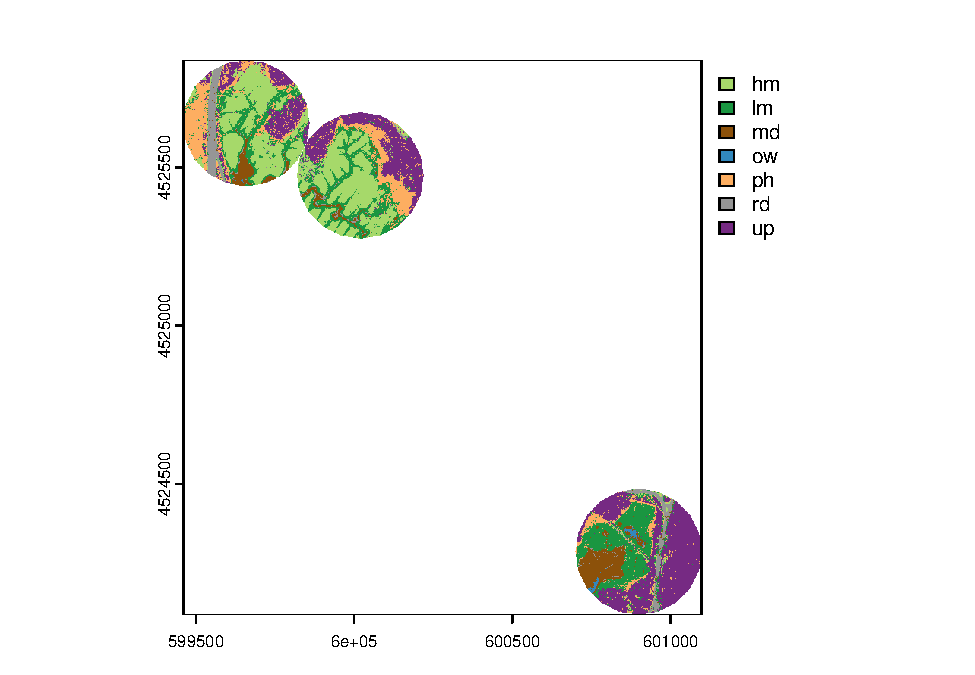
\includegraphics{veg_model_files/figure-latex/unnamed-chunk-8-1.pdf}

\begin{Shaded}
\begin{Highlighting}[]
\CommentTok{\# save the output tif}
\CommentTok{\# writeRaster(classified, "\textasciitilde{}/Desktop/marshbirdsoutput/round\_5/classified\_output.tif", overwrite = TRUE)}

\NormalTok{model }\OtherTok{\textless{}{-}}\NormalTok{ rf\_model}\SpecialCharTok{$}\NormalTok{importance}
\FunctionTok{print}\NormalTok{(model)}
\end{Highlighting}
\end{Shaded}

\begin{verbatim}
##       MeanDecreaseGini
## naip1         1183.124
## naip2         1291.161
## naip3         1724.649
## naip4         1585.792
## ndvi          1803.991
## ndwi          2005.977
\end{verbatim}

\section{feature class importance and
visualizations}\label{feature-class-importance-and-visualizations-1}

\begin{Shaded}
\begin{Highlighting}[]
\FunctionTok{ggplot}\NormalTok{(training\_data, }\FunctionTok{aes}\NormalTok{(}\AttributeTok{x =}\NormalTok{ naip4, }\AttributeTok{y =}\NormalTok{ ndvi, }\AttributeTok{color =}\NormalTok{ class)) }\SpecialCharTok{+}
  \FunctionTok{geom\_point}\NormalTok{(}\AttributeTok{alpha =} \FloatTok{0.3}\NormalTok{) }\SpecialCharTok{+}
  \FunctionTok{theme\_minimal}\NormalTok{()}
\end{Highlighting}
\end{Shaded}

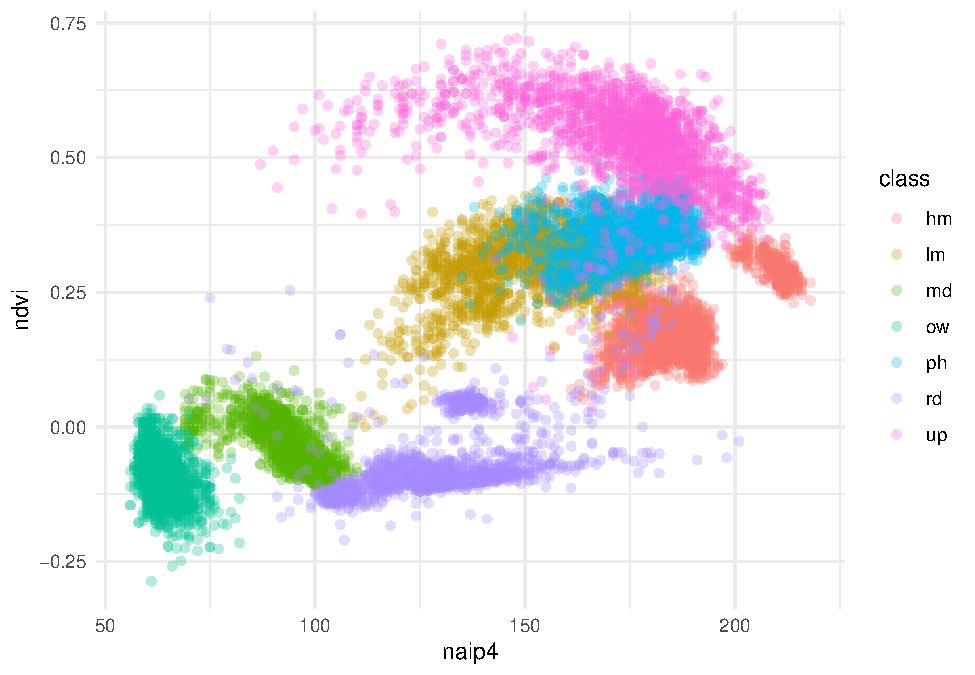
\includegraphics{veg_model_files/figure-latex/unnamed-chunk-9-1.pdf}

\begin{Shaded}
\begin{Highlighting}[]
\FunctionTok{ggplot}\NormalTok{(training\_data, }\FunctionTok{aes}\NormalTok{(}\AttributeTok{x =}\NormalTok{ naip4, }\AttributeTok{fill =}\NormalTok{ class)) }\SpecialCharTok{+}
  \FunctionTok{geom\_density}\NormalTok{(}\AttributeTok{alpha =} \FloatTok{0.4}\NormalTok{, }\AttributeTok{color =} \ConstantTok{NA}\NormalTok{) }\SpecialCharTok{+}
  \FunctionTok{theme\_minimal}\NormalTok{()}
\end{Highlighting}
\end{Shaded}

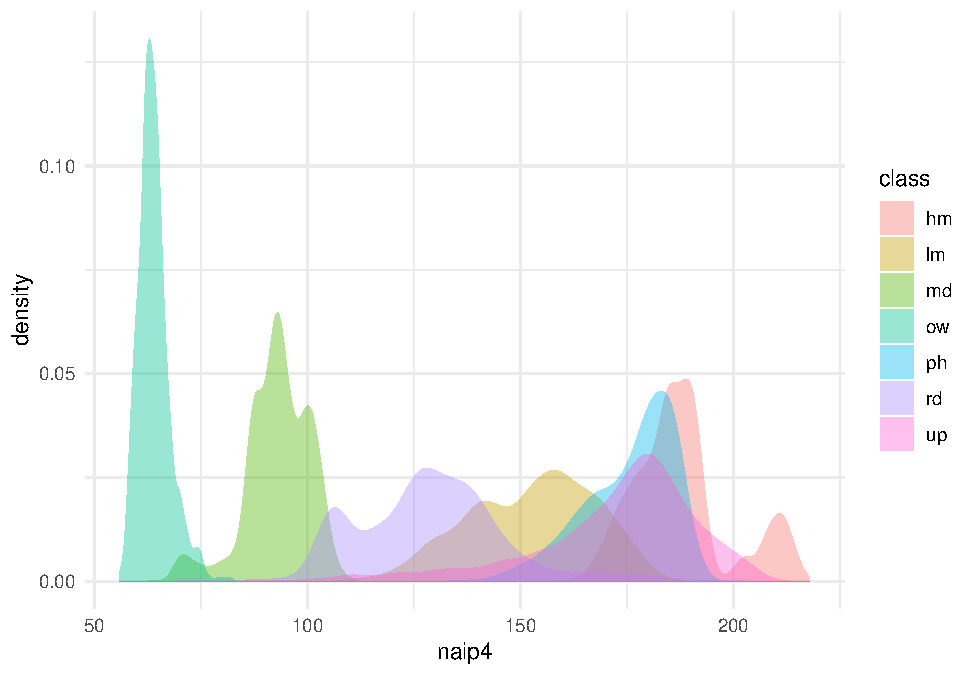
\includegraphics{veg_model_files/figure-latex/unnamed-chunk-9-2.pdf}

\begin{Shaded}
\begin{Highlighting}[]
\NormalTok{imp }\OtherTok{\textless{}{-}} \FunctionTok{as.data.frame}\NormalTok{(rf\_model}\SpecialCharTok{$}\NormalTok{importance)}
\NormalTok{imp}\SpecialCharTok{$}\NormalTok{feature }\OtherTok{\textless{}{-}} \FunctionTok{rownames}\NormalTok{(imp)}

\FunctionTok{ggplot}\NormalTok{(imp, }\FunctionTok{aes}\NormalTok{(}\AttributeTok{x =} \FunctionTok{reorder}\NormalTok{(feature, MeanDecreaseGini), }\AttributeTok{y =}\NormalTok{ MeanDecreaseGini)) }\SpecialCharTok{+}
  \FunctionTok{geom\_col}\NormalTok{(}\AttributeTok{fill =} \StringTok{"steelblue"}\NormalTok{) }\SpecialCharTok{+}
  \FunctionTok{coord\_flip}\NormalTok{() }\SpecialCharTok{+}
  \FunctionTok{labs}\NormalTok{(}\AttributeTok{title =} \StringTok{"Random Forest Variable Importance"}\NormalTok{,}
       \AttributeTok{x =} \StringTok{"Feature"}\NormalTok{, }\AttributeTok{y =} \StringTok{"Mean Decrease Gini"}\NormalTok{) }\SpecialCharTok{+}
  \FunctionTok{theme\_minimal}\NormalTok{()}
\end{Highlighting}
\end{Shaded}

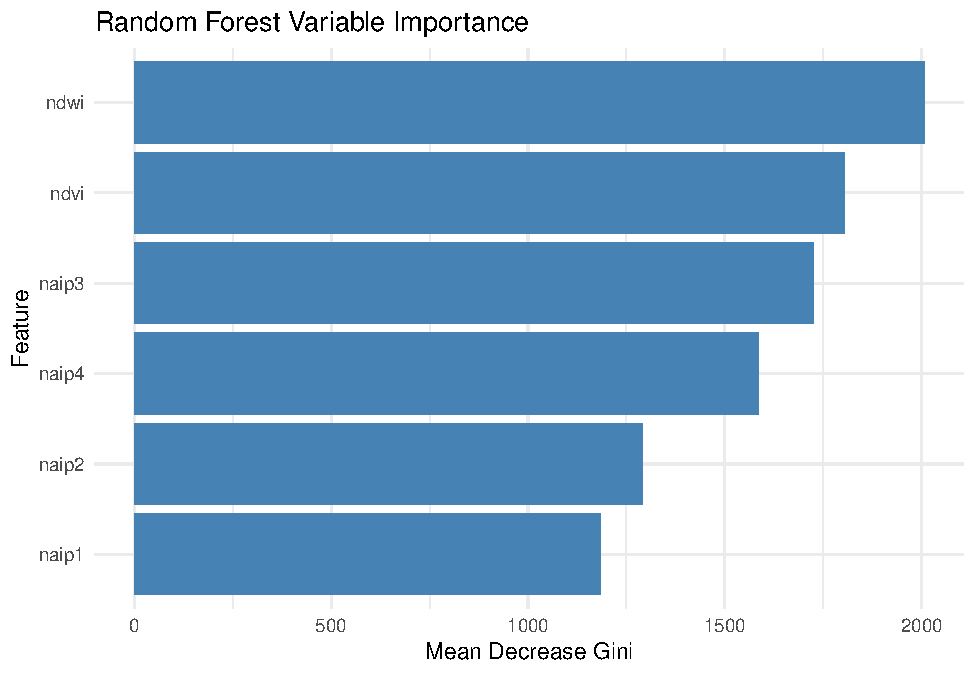
\includegraphics{veg_model_files/figure-latex/unnamed-chunk-9-3.pdf}

\section{3. Third Iteration: NAIP +
NDVI}\label{third-iteration-naip-ndvi}

\begin{Shaded}
\begin{Highlighting}[]
\CommentTok{\# stack em up}
\NormalTok{r\_stack }\OtherTok{\textless{}{-}} \FunctionTok{c}\NormalTok{(naip, ndvi)}

\CommentTok{\# extract raster values for training polygons}
\NormalTok{extracted }\OtherTok{\textless{}{-}}\NormalTok{ terra}\SpecialCharTok{::}\FunctionTok{extract}\NormalTok{(r\_stack, training\_polygons, }\AttributeTok{df =} \ConstantTok{TRUE}\NormalTok{)}

\CommentTok{\# turn class into a factor}
\NormalTok{training\_polygons}\SpecialCharTok{$}\NormalTok{class }\OtherTok{\textless{}{-}} \FunctionTok{as.factor}\NormalTok{(training\_polygons}\SpecialCharTok{$}\NormalTok{class)}

\CommentTok{\# Convert training\_polygons to dataframe to get the class labels}
\NormalTok{poly\_df }\OtherTok{\textless{}{-}} \FunctionTok{as.data.frame}\NormalTok{(training\_polygons)}
\NormalTok{poly\_df}\SpecialCharTok{$}\NormalTok{ID }\OtherTok{\textless{}{-}} \DecValTok{1}\SpecialCharTok{:}\FunctionTok{nrow}\NormalTok{(poly\_df)  }\CommentTok{\# Add ID column to match extract output}

\CommentTok{\# Join the class labels}
\NormalTok{extracted }\OtherTok{\textless{}{-}}\NormalTok{ extracted }\SpecialCharTok{\%\textgreater{}\%}
  \FunctionTok{left\_join}\NormalTok{(poly\_df[, }\FunctionTok{c}\NormalTok{(}\StringTok{"ID"}\NormalTok{, }\StringTok{"class"}\NormalTok{)], }\AttributeTok{by =} \StringTok{"ID"}\NormalTok{)}

\CommentTok{\# clean data by removing rows with na values and remove ID column}
\NormalTok{extracted\_clean }\OtherTok{\textless{}{-}} \FunctionTok{na.omit}\NormalTok{(extracted[, }\SpecialCharTok{{-}}\DecValTok{1}\NormalTok{])  }\CommentTok{\# remove ID and NAs}

\CommentTok{\# sample 2000 per class}
\NormalTok{training\_data }\OtherTok{\textless{}{-}}\NormalTok{ extracted\_clean }\SpecialCharTok{\%\textgreater{}\%}
  \FunctionTok{group\_by}\NormalTok{(class) }\SpecialCharTok{\%\textgreater{}\%}
  \FunctionTok{sample\_n}\NormalTok{(}\FunctionTok{min}\NormalTok{(}\DecValTok{2000}\NormalTok{, }\FunctionTok{n}\NormalTok{())) }\SpecialCharTok{\%\textgreater{}\%}  \CommentTok{\# Use min() to handle small classes}
  \FunctionTok{ungroup}\NormalTok{()}

\CommentTok{\# turn class column into factor}
\NormalTok{training\_data}\SpecialCharTok{$}\NormalTok{class }\OtherTok{\textless{}{-}} \FunctionTok{factor}\NormalTok{(training\_data}\SpecialCharTok{$}\NormalTok{class)}
\end{Highlighting}
\end{Shaded}

\begin{Shaded}
\begin{Highlighting}[]
\CommentTok{\# split training and test data}
\FunctionTok{set.seed}\NormalTok{(}\DecValTok{342}\NormalTok{)}
\NormalTok{idx }\OtherTok{\textless{}{-}} \FunctionTok{sample}\NormalTok{(}\FunctionTok{seq\_len}\NormalTok{(}\FunctionTok{nrow}\NormalTok{(training\_data)), }\AttributeTok{size =} \FloatTok{0.8} \SpecialCharTok{*} \FunctionTok{nrow}\NormalTok{(training\_data))}
\NormalTok{train\_set }\OtherTok{\textless{}{-}}\NormalTok{ training\_data[idx, ]}
\NormalTok{test\_set  }\OtherTok{\textless{}{-}}\NormalTok{ training\_data[}\SpecialCharTok{{-}}\NormalTok{idx, ]}

\CommentTok{\# train random forest model}
\NormalTok{rf\_model }\OtherTok{\textless{}{-}} \FunctionTok{randomForest}\NormalTok{(class }\SpecialCharTok{\textasciitilde{}}\NormalTok{ ., }
                         \AttributeTok{data =}\NormalTok{ train\_set, }
                         \AttributeTok{ntree =} \DecValTok{500}\NormalTok{)}

\CommentTok{\# validation metrics}
\NormalTok{preds }\OtherTok{\textless{}{-}} \FunctionTok{predict}\NormalTok{(rf\_model, }\AttributeTok{newdata =}\NormalTok{ test\_set)}
\NormalTok{accuracy }\OtherTok{\textless{}{-}} \FunctionTok{mean}\NormalTok{(preds }\SpecialCharTok{==}\NormalTok{ test\_set}\SpecialCharTok{$}\NormalTok{class)}
\FunctionTok{cat}\NormalTok{(}\StringTok{"Accuracy:"}\NormalTok{, }\FunctionTok{round}\NormalTok{(accuracy, }\DecValTok{4}\NormalTok{), }\StringTok{"}\SpecialCharTok{\textbackslash{}n}\StringTok{"}\NormalTok{)}
\end{Highlighting}
\end{Shaded}

\begin{verbatim}
## Accuracy: 0.9821
\end{verbatim}

\begin{Shaded}
\begin{Highlighting}[]
\FunctionTok{print}\NormalTok{(rf\_model)}
\end{Highlighting}
\end{Shaded}

\begin{verbatim}
## 
## Call:
##  randomForest(formula = class ~ ., data = train_set, ntree = 500) 
##                Type of random forest: classification
##                      Number of trees: 500
## No. of variables tried at each split: 2
## 
##         OOB estimate of  error rate: 2.26%
## Confusion matrix:
##      hm   lm   md   ow   ph   rd   up class.error
## hm 1597   10    0    0    0    0    0 0.006222775
## lm   15 1538    0    0   40    3    1 0.036944271
## md    0    0 1594    0    0    7    0 0.004372267
## ow    0    0    1 1587    0    1    0 0.001258653
## ph    1   61    0    0 1537    3   10 0.046526055
## rd    9    4   23    0   11 1558    0 0.029283489
## up    2   26    0    0   22    3 1536 0.033354311
\end{verbatim}

\begin{Shaded}
\begin{Highlighting}[]
\CommentTok{\# confusion matrix}
\FunctionTok{confusionMatrix}\NormalTok{(preds, test\_set}\SpecialCharTok{$}\NormalTok{class)}
\end{Highlighting}
\end{Shaded}

\begin{verbatim}
## Confusion Matrix and Statistics
## 
##           Reference
## Prediction  hm  lm  md  ow  ph  rd  up
##         hm 391   5   0   0   0   0   1
##         lm   2 387   0   0  11   1   4
##         md   0   0 399   0   0   3   0
##         ow   0   0   0 411   0   0   0
##         ph   0   9   0   0 376   6   4
##         rd   0   1   0   0   0 385   1
##         up   0   1   0   0   1   0 401
## 
## Overall Statistics
##                                           
##                Accuracy : 0.9821          
##                  95% CI : (0.9765, 0.9867)
##     No Information Rate : 0.1468          
##     P-Value [Acc > NIR] : < 2.2e-16       
##                                           
##                   Kappa : 0.9792          
##                                           
##  Mcnemar's Test P-Value : NA              
## 
## Statistics by Class:
## 
##                      Class: hm Class: lm Class: md Class: ow Class: ph
## Sensitivity             0.9949    0.9603    1.0000    1.0000    0.9691
## Specificity             0.9975    0.9925    0.9988    1.0000    0.9921
## Pos Pred Value          0.9849    0.9556    0.9925    1.0000    0.9519
## Neg Pred Value          0.9992    0.9933    1.0000    1.0000    0.9950
## Prevalence              0.1404    0.1439    0.1425    0.1468    0.1386
## Detection Rate          0.1396    0.1382    0.1425    0.1468    0.1343
## Detection Prevalence    0.1418    0.1446    0.1436    0.1468    0.1411
## Balanced Accuracy       0.9962    0.9764    0.9994    1.0000    0.9806
##                      Class: rd Class: up
## Sensitivity             0.9747    0.9757
## Specificity             0.9992    0.9992
## Pos Pred Value          0.9948    0.9950
## Neg Pred Value          0.9959    0.9958
## Prevalence              0.1411    0.1468
## Detection Rate          0.1375    0.1432
## Detection Prevalence    0.1382    0.1439
## Balanced Accuracy       0.9869    0.9874
\end{verbatim}

\section{classifying the plots}\label{classifying-the-plots-2}

\begin{Shaded}
\begin{Highlighting}[]
\CommentTok{\# load the new, unlabeled raster}
\NormalTok{prediction\_raster }\OtherTok{\textless{}{-}} \FunctionTok{rast}\NormalTok{(}\StringTok{"\textasciitilde{}/Desktop/marshbirdsoutput/round\_5/prediction\_raster\_round\_5.tif"}\NormalTok{)}

\CommentTok{\# calculate NDVI for prediction raster}
\NormalTok{ndvi\_pred }\OtherTok{\textless{}{-}}\NormalTok{ (prediction\_raster[[}\DecValTok{4}\NormalTok{]] }\SpecialCharTok{{-}}\NormalTok{ prediction\_raster[[}\DecValTok{1}\NormalTok{]]) }\SpecialCharTok{/} 
\NormalTok{  (prediction\_raster[[}\DecValTok{4}\NormalTok{]] }\SpecialCharTok{+}\NormalTok{ prediction\_raster[[}\DecValTok{1}\NormalTok{]])}
\FunctionTok{names}\NormalTok{(ndvi\_pred) }\OtherTok{\textless{}{-}} \StringTok{"ndvi"}

\CommentTok{\# calculation NDWI}
\NormalTok{ndwi\_pred }\OtherTok{\textless{}{-}}\NormalTok{ (prediction\_raster[[}\DecValTok{4}\NormalTok{]] }\SpecialCharTok{{-}}\NormalTok{ prediction\_raster[[}\DecValTok{2}\NormalTok{]]) }\SpecialCharTok{/} 
\NormalTok{  (prediction\_raster[[}\DecValTok{4}\NormalTok{]] }\SpecialCharTok{+}\NormalTok{ prediction\_raster[[}\DecValTok{2}\NormalTok{]])}
\FunctionTok{names}\NormalTok{(ndwi\_pred) }\OtherTok{\textless{}{-}} \StringTok{"ndwi"}

\CommentTok{\# Calculate brightness}
\NormalTok{brightness\_pred }\OtherTok{\textless{}{-}}\NormalTok{ (prediction\_raster[[}\DecValTok{1}\NormalTok{]] }\SpecialCharTok{+}\NormalTok{ prediction\_raster[[}\DecValTok{2}\NormalTok{]] }\SpecialCharTok{+} 
\NormalTok{                      prediction\_raster[[}\DecValTok{3}\NormalTok{]] }\SpecialCharTok{+}\NormalTok{ prediction\_raster[[}\DecValTok{4}\NormalTok{]]) }\SpecialCharTok{/} \DecValTok{4}
\FunctionTok{names}\NormalTok{(brightness\_pred) }\OtherTok{\textless{}{-}} \StringTok{"brightness"}

\CommentTok{\# Apply the pca}
\NormalTok{all\_for\_pca\_pred }\OtherTok{\textless{}{-}} \FunctionTok{c}\NormalTok{(prediction\_raster, ndvi\_pred)}
\FunctionTok{names}\NormalTok{(all\_for\_pca\_pred) }\OtherTok{\textless{}{-}} \FunctionTok{names}\NormalTok{(all\_for\_pca)  }\CommentTok{\# ensure exact match}
\NormalTok{pca\_pred }\OtherTok{\textless{}{-}} \FunctionTok{predict}\NormalTok{(all\_for\_pca\_pred, pca\_pixels, }\AttributeTok{index =} \DecValTok{1}\SpecialCharTok{:}\DecValTok{5}\NormalTok{)}
\end{Highlighting}
\end{Shaded}

\begin{verbatim}
## |---------|---------|---------|---------|=========================================                                          
\end{verbatim}

\begin{Shaded}
\begin{Highlighting}[]
\FunctionTok{names}\NormalTok{(pca\_pred) }\OtherTok{\textless{}{-}} \FunctionTok{paste0}\NormalTok{(}\StringTok{"PCA"}\NormalTok{, }\DecValTok{1}\SpecialCharTok{:}\DecValTok{5}\NormalTok{)}

\CommentTok{\# stack it}
\NormalTok{prediction\_stack }\OtherTok{\textless{}{-}} \FunctionTok{c}\NormalTok{(prediction\_raster, ndvi\_pred)}

\CommentTok{\# rename to match training names}
\FunctionTok{names}\NormalTok{(prediction\_stack) }\OtherTok{\textless{}{-}} \FunctionTok{names}\NormalTok{(r\_stack)}

\CommentTok{\# apply the model to predict classes}
\NormalTok{classified }\OtherTok{\textless{}{-}} \FunctionTok{predict}\NormalTok{(prediction\_stack, rf\_model, }\AttributeTok{na.rm =} \ConstantTok{TRUE}\NormalTok{)}

\CommentTok{\# Define custom colors}
\NormalTok{colors }\OtherTok{\textless{}{-}} \FunctionTok{c}\NormalTok{(}
  \StringTok{"\#a6d96a"}\NormalTok{,  }\CommentTok{\# hm  }
  \StringTok{"\#1a9641"}\NormalTok{,  }\CommentTok{\# lm  }
  \StringTok{"\#8c510a"}\NormalTok{,  }\CommentTok{\# md  }
  \StringTok{"\#3288bd"}\NormalTok{,  }\CommentTok{\# ow  }
  \StringTok{"\#fdae61"}\NormalTok{,  }\CommentTok{\# ph  }
  \StringTok{"\#969696"}\NormalTok{,  }\CommentTok{\# rd  }
  \StringTok{"\#762a83"}   \CommentTok{\# up  }
\NormalTok{)}



\CommentTok{\# Plot with colors}
\FunctionTok{plot}\NormalTok{(classified, }\AttributeTok{col =}\NormalTok{ colors)}
\end{Highlighting}
\end{Shaded}

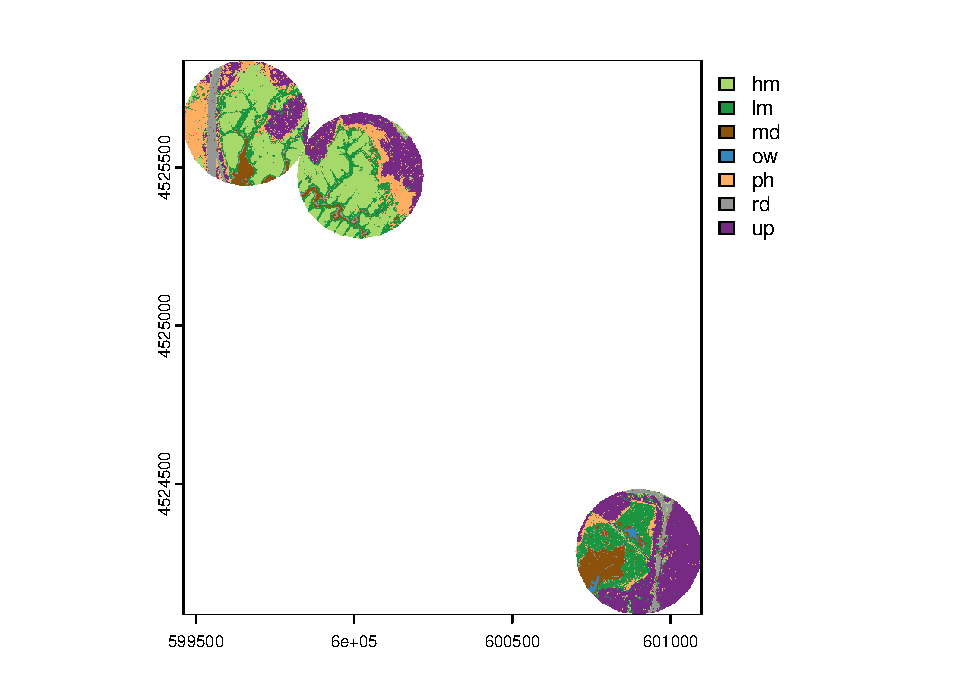
\includegraphics{veg_model_files/figure-latex/unnamed-chunk-12-1.pdf}

\begin{Shaded}
\begin{Highlighting}[]
\CommentTok{\# save the output tif}
\FunctionTok{writeRaster}\NormalTok{(classified, }\StringTok{"\textasciitilde{}/Desktop/marshbirdsoutput/round\_5/classified\_output.tif"}\NormalTok{, }\AttributeTok{overwrite =} \ConstantTok{TRUE}\NormalTok{)}

\NormalTok{rf\_model}\SpecialCharTok{$}\NormalTok{importance}
\end{Highlighting}
\end{Shaded}

\begin{verbatim}
##       MeanDecreaseGini
## naip1         1461.871
## naip2         1427.051
## naip3         1937.398
## naip4         2257.483
## ndvi          2510.155
\end{verbatim}

\section{feature class importance and
visualizations}\label{feature-class-importance-and-visualizations-2}

\begin{Shaded}
\begin{Highlighting}[]
\FunctionTok{ggplot}\NormalTok{(training\_data, }\FunctionTok{aes}\NormalTok{(}\AttributeTok{x =}\NormalTok{ naip4, }\AttributeTok{y =}\NormalTok{ ndvi, }\AttributeTok{color =}\NormalTok{ class)) }\SpecialCharTok{+}
  \FunctionTok{geom\_point}\NormalTok{(}\AttributeTok{alpha =} \FloatTok{0.3}\NormalTok{) }\SpecialCharTok{+}
  \FunctionTok{theme\_minimal}\NormalTok{()}
\end{Highlighting}
\end{Shaded}

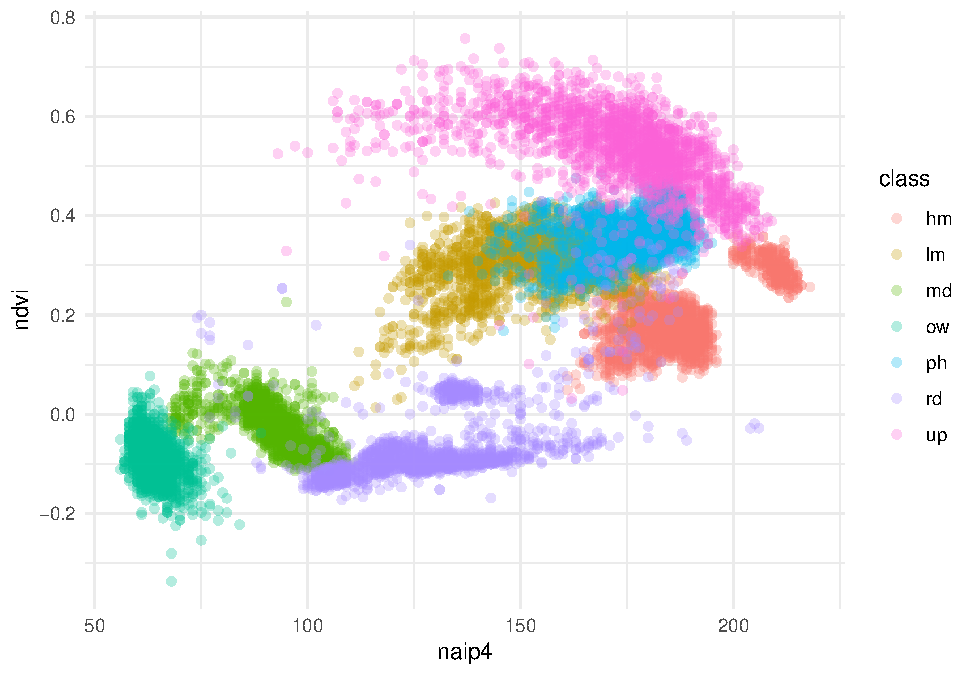
\includegraphics{veg_model_files/figure-latex/unnamed-chunk-13-1.pdf}

\begin{Shaded}
\begin{Highlighting}[]
\FunctionTok{ggplot}\NormalTok{(training\_data, }\FunctionTok{aes}\NormalTok{(}\AttributeTok{x =}\NormalTok{ naip4, }\AttributeTok{fill =}\NormalTok{ class)) }\SpecialCharTok{+}
  \FunctionTok{geom\_density}\NormalTok{(}\AttributeTok{alpha =} \FloatTok{0.4}\NormalTok{, }\AttributeTok{color =} \ConstantTok{NA}\NormalTok{) }\SpecialCharTok{+}
  \FunctionTok{theme\_minimal}\NormalTok{()}
\end{Highlighting}
\end{Shaded}

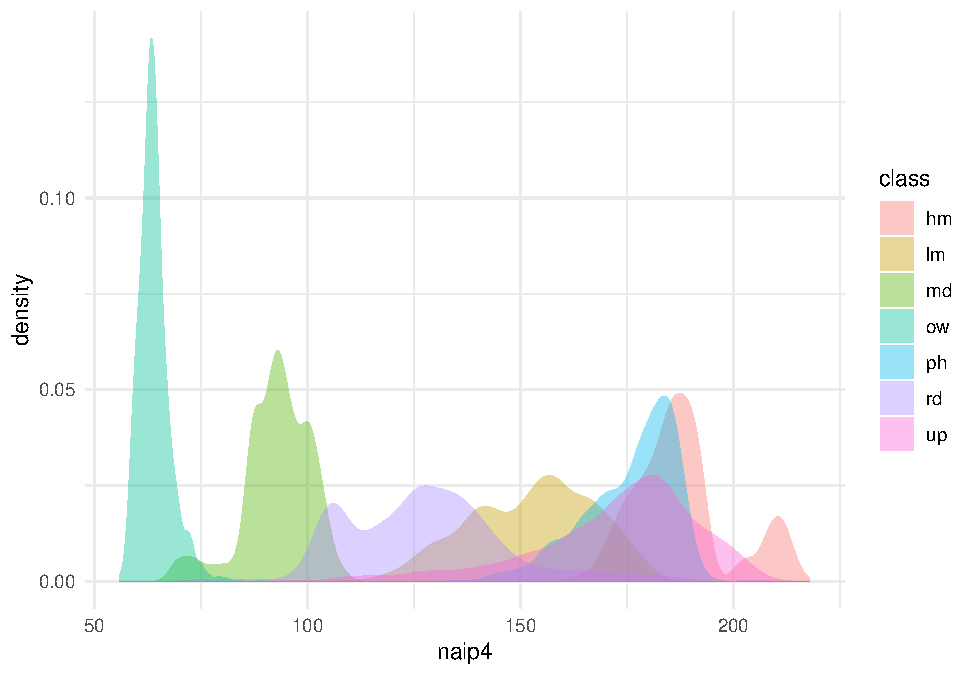
\includegraphics{veg_model_files/figure-latex/unnamed-chunk-13-2.pdf}

\begin{Shaded}
\begin{Highlighting}[]
\NormalTok{imp }\OtherTok{\textless{}{-}} \FunctionTok{as.data.frame}\NormalTok{(rf\_model}\SpecialCharTok{$}\NormalTok{importance)}
\NormalTok{imp}\SpecialCharTok{$}\NormalTok{feature }\OtherTok{\textless{}{-}} \FunctionTok{rownames}\NormalTok{(imp)}

\FunctionTok{ggplot}\NormalTok{(imp, }\FunctionTok{aes}\NormalTok{(}\AttributeTok{x =} \FunctionTok{reorder}\NormalTok{(feature, MeanDecreaseGini), }\AttributeTok{y =}\NormalTok{ MeanDecreaseGini)) }\SpecialCharTok{+}
  \FunctionTok{geom\_col}\NormalTok{(}\AttributeTok{fill =} \StringTok{"steelblue"}\NormalTok{) }\SpecialCharTok{+}
  \FunctionTok{coord\_flip}\NormalTok{() }\SpecialCharTok{+}
  \FunctionTok{labs}\NormalTok{(}\AttributeTok{title =} \StringTok{"Random Forest Variable Importance"}\NormalTok{,}
       \AttributeTok{x =} \StringTok{"Feature"}\NormalTok{, }\AttributeTok{y =} \StringTok{"Mean Decrease Gini"}\NormalTok{) }\SpecialCharTok{+}
  \FunctionTok{theme\_minimal}\NormalTok{()}
\end{Highlighting}
\end{Shaded}

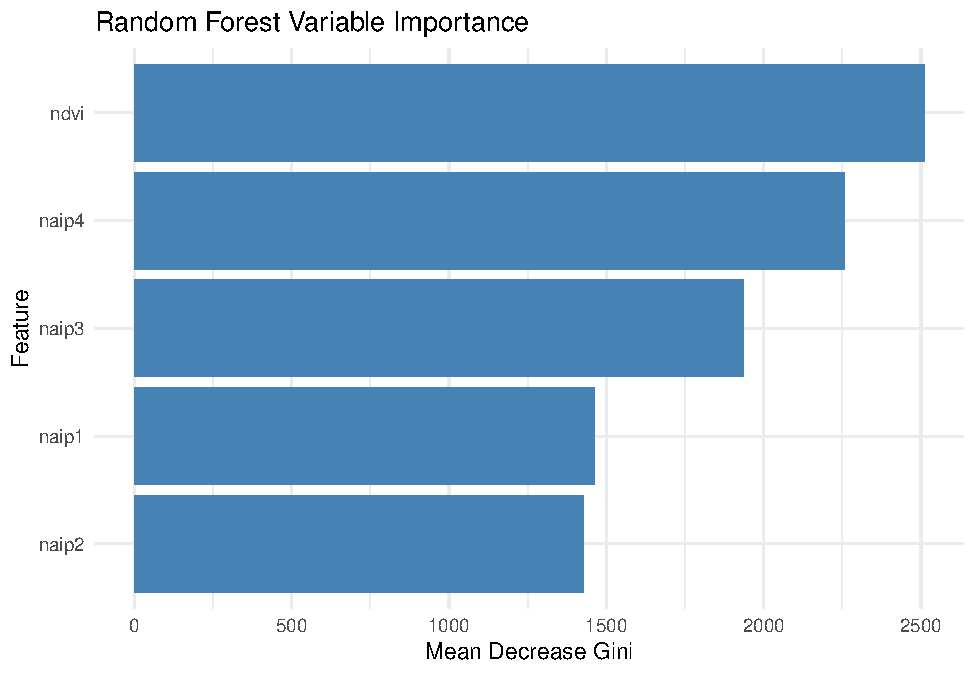
\includegraphics{veg_model_files/figure-latex/unnamed-chunk-13-3.pdf}

\section{4. Fourth Iteration: PCA}\label{fourth-iteration-pca}

\begin{Shaded}
\begin{Highlighting}[]
\CommentTok{\# stack em up}
\NormalTok{r\_stack }\OtherTok{\textless{}{-}} \FunctionTok{c}\NormalTok{(pca)}

\CommentTok{\# extract raster values for training polygons}
\NormalTok{extracted }\OtherTok{\textless{}{-}}\NormalTok{ terra}\SpecialCharTok{::}\FunctionTok{extract}\NormalTok{(r\_stack, training\_polygons, }\AttributeTok{df =} \ConstantTok{TRUE}\NormalTok{)}

\CommentTok{\# turn class into a factor}
\NormalTok{training\_polygons}\SpecialCharTok{$}\NormalTok{class }\OtherTok{\textless{}{-}} \FunctionTok{as.factor}\NormalTok{(training\_polygons}\SpecialCharTok{$}\NormalTok{class)}

\CommentTok{\# Convert training\_polygons to dataframe to get the class labels}
\NormalTok{poly\_df }\OtherTok{\textless{}{-}} \FunctionTok{as.data.frame}\NormalTok{(training\_polygons)}
\NormalTok{poly\_df}\SpecialCharTok{$}\NormalTok{ID }\OtherTok{\textless{}{-}} \DecValTok{1}\SpecialCharTok{:}\FunctionTok{nrow}\NormalTok{(poly\_df)  }\CommentTok{\# Add ID column to match extract output}

\CommentTok{\# Join the class labels}
\NormalTok{extracted }\OtherTok{\textless{}{-}}\NormalTok{ extracted }\SpecialCharTok{\%\textgreater{}\%}
  \FunctionTok{left\_join}\NormalTok{(poly\_df[, }\FunctionTok{c}\NormalTok{(}\StringTok{"ID"}\NormalTok{, }\StringTok{"class"}\NormalTok{)], }\AttributeTok{by =} \StringTok{"ID"}\NormalTok{)}

\CommentTok{\# clean data by removing rows with na values and remove ID column}
\NormalTok{extracted\_clean }\OtherTok{\textless{}{-}} \FunctionTok{na.omit}\NormalTok{(extracted[, }\SpecialCharTok{{-}}\DecValTok{1}\NormalTok{])  }\CommentTok{\# remove ID and NAs}

\CommentTok{\# sample 2000 per class}
\NormalTok{training\_data }\OtherTok{\textless{}{-}}\NormalTok{ extracted\_clean }\SpecialCharTok{\%\textgreater{}\%}
  \FunctionTok{group\_by}\NormalTok{(class) }\SpecialCharTok{\%\textgreater{}\%}
  \FunctionTok{sample\_n}\NormalTok{(}\FunctionTok{min}\NormalTok{(}\DecValTok{2000}\NormalTok{, }\FunctionTok{n}\NormalTok{())) }\SpecialCharTok{\%\textgreater{}\%}  \CommentTok{\# Use min() to handle small classes}
  \FunctionTok{ungroup}\NormalTok{()}

\CommentTok{\# turn class column into factor}
\NormalTok{training\_data}\SpecialCharTok{$}\NormalTok{class }\OtherTok{\textless{}{-}} \FunctionTok{factor}\NormalTok{(training\_data}\SpecialCharTok{$}\NormalTok{class)}
\end{Highlighting}
\end{Shaded}

\section{check the sampling balance in the
classes}\label{check-the-sampling-balance-in-the-classes}

\section{print(``Class distribution in training
data:'')}\label{printclass-distribution-in-training-data}

\section{print(table(training\_data\$class))}\label{printtabletraining_dataclass}

\begin{Shaded}
\begin{Highlighting}[]
\CommentTok{\# split training and test data}
\FunctionTok{set.seed}\NormalTok{(}\DecValTok{342}\NormalTok{)}
\NormalTok{idx }\OtherTok{\textless{}{-}} \FunctionTok{sample}\NormalTok{(}\FunctionTok{seq\_len}\NormalTok{(}\FunctionTok{nrow}\NormalTok{(training\_data)), }\AttributeTok{size =} \FloatTok{0.8} \SpecialCharTok{*} \FunctionTok{nrow}\NormalTok{(training\_data))}
\NormalTok{train\_set }\OtherTok{\textless{}{-}}\NormalTok{ training\_data[idx, ]}
\NormalTok{test\_set  }\OtherTok{\textless{}{-}}\NormalTok{ training\_data[}\SpecialCharTok{{-}}\NormalTok{idx, ]}

\CommentTok{\# train random forest model}
\NormalTok{rf\_model }\OtherTok{\textless{}{-}} \FunctionTok{randomForest}\NormalTok{(class }\SpecialCharTok{\textasciitilde{}}\NormalTok{ ., }
                         \AttributeTok{data =}\NormalTok{ train\_set, }
                         \AttributeTok{ntree =} \DecValTok{500}\NormalTok{)}

\CommentTok{\# validation metrics}
\NormalTok{preds }\OtherTok{\textless{}{-}} \FunctionTok{predict}\NormalTok{(rf\_model, }\AttributeTok{newdata =}\NormalTok{ test\_set)}
\NormalTok{accuracy }\OtherTok{\textless{}{-}} \FunctionTok{mean}\NormalTok{(preds }\SpecialCharTok{==}\NormalTok{ test\_set}\SpecialCharTok{$}\NormalTok{class)}
\FunctionTok{cat}\NormalTok{(}\StringTok{"Accuracy:"}\NormalTok{, }\FunctionTok{round}\NormalTok{(accuracy, }\DecValTok{4}\NormalTok{), }\StringTok{"}\SpecialCharTok{\textbackslash{}n}\StringTok{"}\NormalTok{)}
\end{Highlighting}
\end{Shaded}

\begin{verbatim}
## Accuracy: 0.9771
\end{verbatim}

\begin{Shaded}
\begin{Highlighting}[]
\FunctionTok{print}\NormalTok{(rf\_model)}
\end{Highlighting}
\end{Shaded}

\begin{verbatim}
## 
## Call:
##  randomForest(formula = class ~ ., data = train_set, ntree = 500) 
##                Type of random forest: classification
##                      Number of trees: 500
## No. of variables tried at each split: 2
## 
##         OOB estimate of  error rate: 1.78%
## Confusion matrix:
##      hm   lm   md   ow   ph   rd   up class.error
## hm 1596    9    0    0    1    1    0 0.006845053
## lm   10 1550    7    0   25    1    4 0.029430182
## md    0    0 1591    2    0    8    0 0.006246096
## ow    0    0    8 1579    0    2    0 0.006293266
## ph    0   40    0    0 1555    1   16 0.035359801
## rd    0    0   13    1   11 1579    1 0.016199377
## up    0   12    0    0   26    0 1551 0.023914412
\end{verbatim}

\begin{Shaded}
\begin{Highlighting}[]
\CommentTok{\# confusion matrix}
\FunctionTok{confusionMatrix}\NormalTok{(preds, test\_set}\SpecialCharTok{$}\NormalTok{class)}
\end{Highlighting}
\end{Shaded}

\begin{verbatim}
## Confusion Matrix and Statistics
## 
##           Reference
## Prediction  hm  lm  md  ow  ph  rd  up
##         hm 388   4   0   0   0   0   1
##         lm   4 387   1   0  15   0   5
##         md   0   1 394   3   0   1   0
##         ow   0   0   2 408   0   0   0
##         ph   0   9   0   0 368   1   7
##         rd   0   0   2   0   1 393   0
##         up   1   2   0   0   4   0 398
## 
## Overall Statistics
##                                           
##                Accuracy : 0.9771          
##                  95% CI : (0.9709, 0.9824)
##     No Information Rate : 0.1468          
##     P-Value [Acc > NIR] : < 2.2e-16       
##                                           
##                   Kappa : 0.9733          
##                                           
##  Mcnemar's Test P-Value : NA              
## 
## Statistics by Class:
## 
##                      Class: hm Class: lm Class: md Class: ow Class: ph
## Sensitivity             0.9873    0.9603    0.9875    0.9927    0.9485
## Specificity             0.9979    0.9896    0.9979    0.9992    0.9930
## Pos Pred Value          0.9873    0.9393    0.9875    0.9951    0.9558
## Neg Pred Value          0.9979    0.9933    0.9979    0.9987    0.9917
## Prevalence              0.1404    0.1439    0.1425    0.1468    0.1386
## Detection Rate          0.1386    0.1382    0.1407    0.1457    0.1314
## Detection Prevalence    0.1404    0.1471    0.1425    0.1464    0.1375
## Balanced Accuracy       0.9926    0.9749    0.9927    0.9959    0.9707
##                      Class: rd Class: up
## Sensitivity             0.9949    0.9684
## Specificity             0.9988    0.9971
## Pos Pred Value          0.9924    0.9827
## Neg Pred Value          0.9992    0.9946
## Prevalence              0.1411    0.1468
## Detection Rate          0.1404    0.1421
## Detection Prevalence    0.1414    0.1446
## Balanced Accuracy       0.9968    0.9827
\end{verbatim}

\section{classifying the plots}\label{classifying-the-plots-3}

\begin{Shaded}
\begin{Highlighting}[]
\CommentTok{\# load the new, unlabeled raster}
\NormalTok{prediction\_raster }\OtherTok{\textless{}{-}} \FunctionTok{rast}\NormalTok{(}\StringTok{"\textasciitilde{}/Desktop/marshbirdsoutput/round\_5/prediction\_raster\_round\_5.tif"}\NormalTok{)}

\CommentTok{\# calculate NDVI for prediction raster}
\NormalTok{ndvi\_pred }\OtherTok{\textless{}{-}}\NormalTok{ (prediction\_raster[[}\DecValTok{4}\NormalTok{]] }\SpecialCharTok{{-}}\NormalTok{ prediction\_raster[[}\DecValTok{1}\NormalTok{]]) }\SpecialCharTok{/} 
\NormalTok{  (prediction\_raster[[}\DecValTok{4}\NormalTok{]] }\SpecialCharTok{+}\NormalTok{ prediction\_raster[[}\DecValTok{1}\NormalTok{]])}
\FunctionTok{names}\NormalTok{(ndvi\_pred) }\OtherTok{\textless{}{-}} \StringTok{"ndvi"}

\CommentTok{\# calculation NDWI}
\NormalTok{ndwi\_pred }\OtherTok{\textless{}{-}}\NormalTok{ (prediction\_raster[[}\DecValTok{4}\NormalTok{]] }\SpecialCharTok{{-}}\NormalTok{ prediction\_raster[[}\DecValTok{2}\NormalTok{]]) }\SpecialCharTok{/} 
\NormalTok{  (prediction\_raster[[}\DecValTok{4}\NormalTok{]] }\SpecialCharTok{+}\NormalTok{ prediction\_raster[[}\DecValTok{2}\NormalTok{]])}
\FunctionTok{names}\NormalTok{(ndwi\_pred) }\OtherTok{\textless{}{-}} \StringTok{"ndwi"}

\CommentTok{\# Calculate brightness}
\NormalTok{brightness\_pred }\OtherTok{\textless{}{-}}\NormalTok{ (prediction\_raster[[}\DecValTok{1}\NormalTok{]] }\SpecialCharTok{+}\NormalTok{ prediction\_raster[[}\DecValTok{2}\NormalTok{]] }\SpecialCharTok{+} 
\NormalTok{                      prediction\_raster[[}\DecValTok{3}\NormalTok{]] }\SpecialCharTok{+}\NormalTok{ prediction\_raster[[}\DecValTok{4}\NormalTok{]]) }\SpecialCharTok{/} \DecValTok{4}
\FunctionTok{names}\NormalTok{(brightness\_pred) }\OtherTok{\textless{}{-}} \StringTok{"brightness"}

\CommentTok{\# Apply the pca}
\NormalTok{all\_for\_pca\_pred }\OtherTok{\textless{}{-}} \FunctionTok{c}\NormalTok{(prediction\_raster, ndvi\_pred)}
\FunctionTok{names}\NormalTok{(all\_for\_pca\_pred) }\OtherTok{\textless{}{-}} \FunctionTok{names}\NormalTok{(all\_for\_pca)  }\CommentTok{\# ensure exact match}
\NormalTok{pca\_pred }\OtherTok{\textless{}{-}} \FunctionTok{predict}\NormalTok{(all\_for\_pca\_pred, pca\_pixels, }\AttributeTok{index =} \DecValTok{1}\SpecialCharTok{:}\DecValTok{5}\NormalTok{)}
\end{Highlighting}
\end{Shaded}

\begin{verbatim}
## |---------|---------|---------|---------|=========================================                                          
\end{verbatim}

\begin{Shaded}
\begin{Highlighting}[]
\FunctionTok{names}\NormalTok{(pca\_pred) }\OtherTok{\textless{}{-}} \FunctionTok{paste0}\NormalTok{(}\StringTok{"PCA"}\NormalTok{, }\DecValTok{1}\SpecialCharTok{:}\DecValTok{5}\NormalTok{)}

\CommentTok{\# stack it}
\NormalTok{prediction\_stack }\OtherTok{\textless{}{-}} \FunctionTok{c}\NormalTok{(pca\_pred)}

\CommentTok{\# rename to match training names}
\FunctionTok{names}\NormalTok{(prediction\_stack) }\OtherTok{\textless{}{-}} \FunctionTok{names}\NormalTok{(r\_stack)}

\CommentTok{\# apply the model to predict classes}
\NormalTok{classified }\OtherTok{\textless{}{-}} \FunctionTok{predict}\NormalTok{(prediction\_stack, rf\_model, }\AttributeTok{na.rm =} \ConstantTok{TRUE}\NormalTok{)}

\CommentTok{\# Define custom colors}
\NormalTok{colors }\OtherTok{\textless{}{-}} \FunctionTok{c}\NormalTok{(}
  \StringTok{"\#a6d96a"}\NormalTok{,  }\CommentTok{\# hm  }
  \StringTok{"\#1a9641"}\NormalTok{,  }\CommentTok{\# lm  }
  \StringTok{"\#8c510a"}\NormalTok{,  }\CommentTok{\# md  }
  \StringTok{"\#3288bd"}\NormalTok{,  }\CommentTok{\# ow  }
  \StringTok{"\#fdae61"}\NormalTok{,  }\CommentTok{\# ph  }
  \StringTok{"\#969696"}\NormalTok{,  }\CommentTok{\# rd  }
  \StringTok{"\#762a83"}   \CommentTok{\# up  }
\NormalTok{)}



\CommentTok{\# Plot with colors}
\FunctionTok{plot}\NormalTok{(classified, }\AttributeTok{col =}\NormalTok{ colors)}
\end{Highlighting}
\end{Shaded}

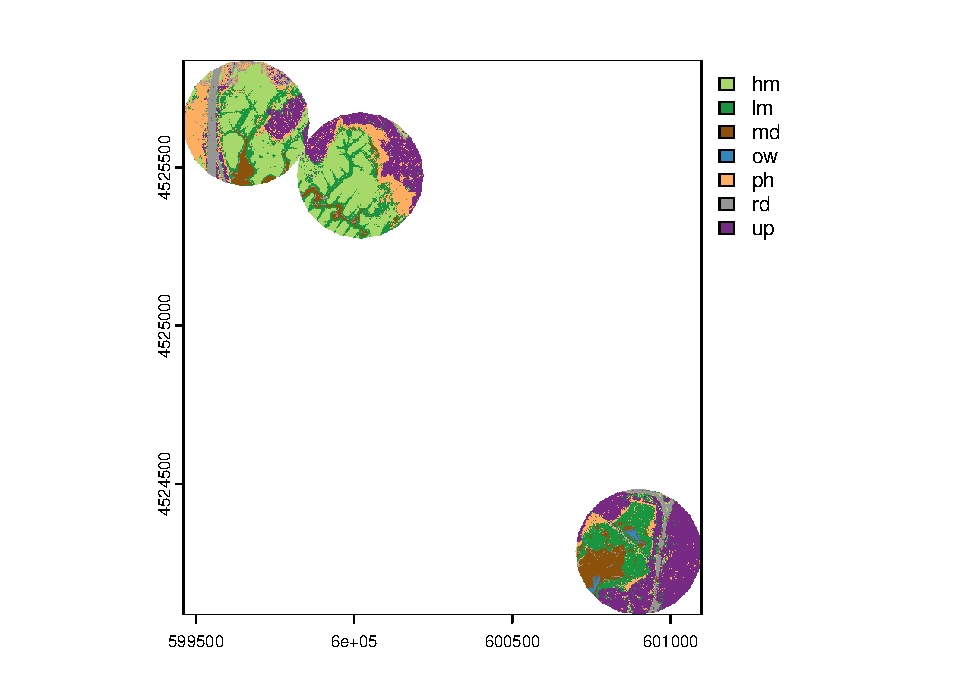
\includegraphics{veg_model_files/figure-latex/unnamed-chunk-16-1.pdf}

\begin{Shaded}
\begin{Highlighting}[]
\CommentTok{\# save the output tif}
\FunctionTok{writeRaster}\NormalTok{(classified, }\StringTok{"\textasciitilde{}/Desktop/marshbirdsoutput/round\_5/classified\_output.tif"}\NormalTok{, }\AttributeTok{overwrite =} \ConstantTok{TRUE}\NormalTok{)}

\NormalTok{rf\_model}\SpecialCharTok{$}\NormalTok{importance}
\end{Highlighting}
\end{Shaded}

\begin{verbatim}
##      MeanDecreaseGini
## PCA1        3351.2342
## PCA2        2768.7772
## PCA3        1786.6728
## PCA4         838.4614
## PCA5         854.0149
\end{verbatim}

\section{feature class importance and
visualizations}\label{feature-class-importance-and-visualizations-3}

\begin{Shaded}
\begin{Highlighting}[]
\FunctionTok{ggplot}\NormalTok{(training\_data, }\FunctionTok{aes}\NormalTok{(}\AttributeTok{x =}\NormalTok{ PCA3, }\AttributeTok{y =}\NormalTok{ PCA1, }\AttributeTok{color =}\NormalTok{ class)) }\SpecialCharTok{+}
  \FunctionTok{geom\_point}\NormalTok{(}\AttributeTok{alpha =} \FloatTok{0.3}\NormalTok{) }\SpecialCharTok{+}
  \FunctionTok{theme\_minimal}\NormalTok{()}
\end{Highlighting}
\end{Shaded}

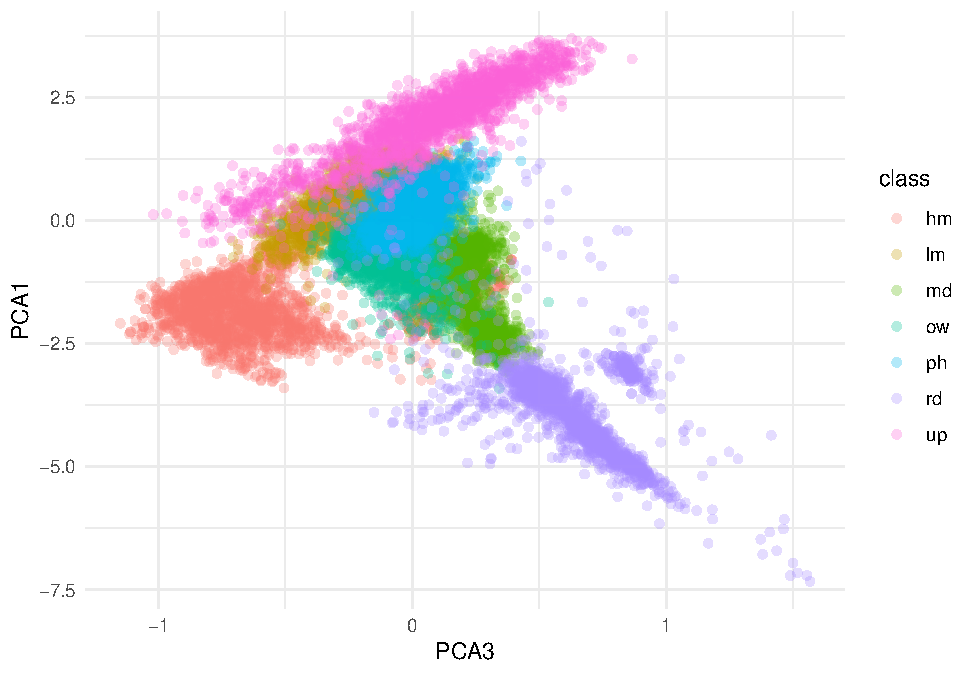
\includegraphics{veg_model_files/figure-latex/unnamed-chunk-17-1.pdf}

\begin{Shaded}
\begin{Highlighting}[]
\FunctionTok{ggplot}\NormalTok{(training\_data, }\FunctionTok{aes}\NormalTok{(}\AttributeTok{x =}\NormalTok{ PCA1, }\AttributeTok{fill =}\NormalTok{ class)) }\SpecialCharTok{+}
  \FunctionTok{geom\_density}\NormalTok{(}\AttributeTok{alpha =} \FloatTok{0.4}\NormalTok{, }\AttributeTok{color =} \ConstantTok{NA}\NormalTok{) }\SpecialCharTok{+}
  \FunctionTok{theme\_minimal}\NormalTok{()}
\end{Highlighting}
\end{Shaded}

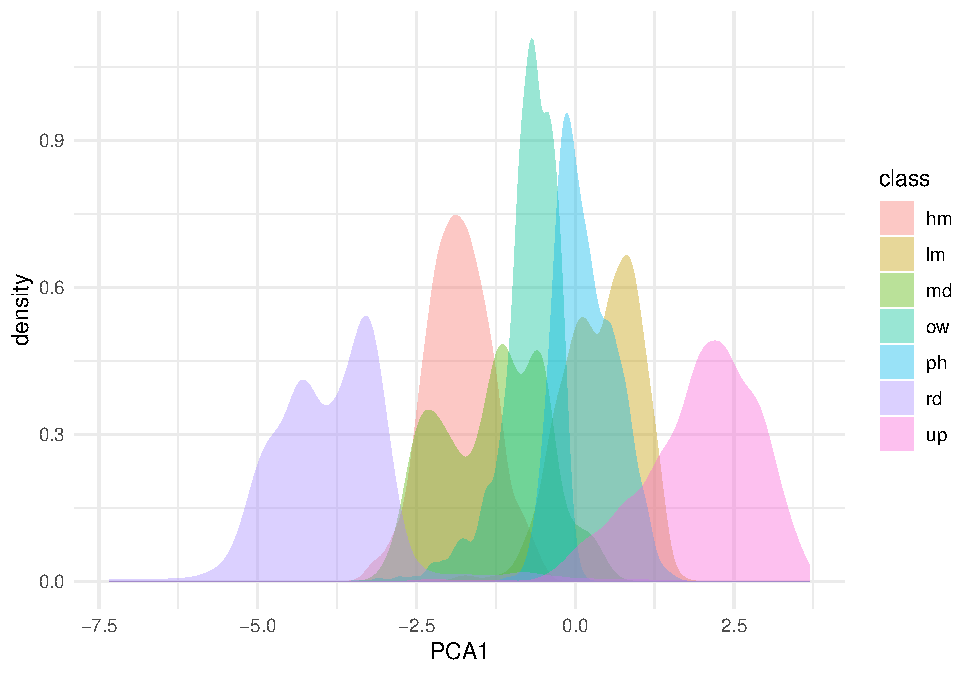
\includegraphics{veg_model_files/figure-latex/unnamed-chunk-17-2.pdf}

\begin{Shaded}
\begin{Highlighting}[]
\NormalTok{imp }\OtherTok{\textless{}{-}} \FunctionTok{as.data.frame}\NormalTok{(rf\_model}\SpecialCharTok{$}\NormalTok{importance)}
\NormalTok{imp}\SpecialCharTok{$}\NormalTok{feature }\OtherTok{\textless{}{-}} \FunctionTok{rownames}\NormalTok{(imp)}

\FunctionTok{ggplot}\NormalTok{(imp, }\FunctionTok{aes}\NormalTok{(}\AttributeTok{x =} \FunctionTok{reorder}\NormalTok{(feature, MeanDecreaseGini), }\AttributeTok{y =}\NormalTok{ MeanDecreaseGini)) }\SpecialCharTok{+}
  \FunctionTok{geom\_col}\NormalTok{(}\AttributeTok{fill =} \StringTok{"steelblue"}\NormalTok{) }\SpecialCharTok{+}
  \FunctionTok{coord\_flip}\NormalTok{() }\SpecialCharTok{+}
  \FunctionTok{labs}\NormalTok{(}\AttributeTok{title =} \StringTok{"Random Forest Variable Importance"}\NormalTok{,}
       \AttributeTok{x =} \StringTok{"Feature"}\NormalTok{, }\AttributeTok{y =} \StringTok{"Mean Decrease Gini"}\NormalTok{) }\SpecialCharTok{+}
  \FunctionTok{theme\_minimal}\NormalTok{()}
\end{Highlighting}
\end{Shaded}

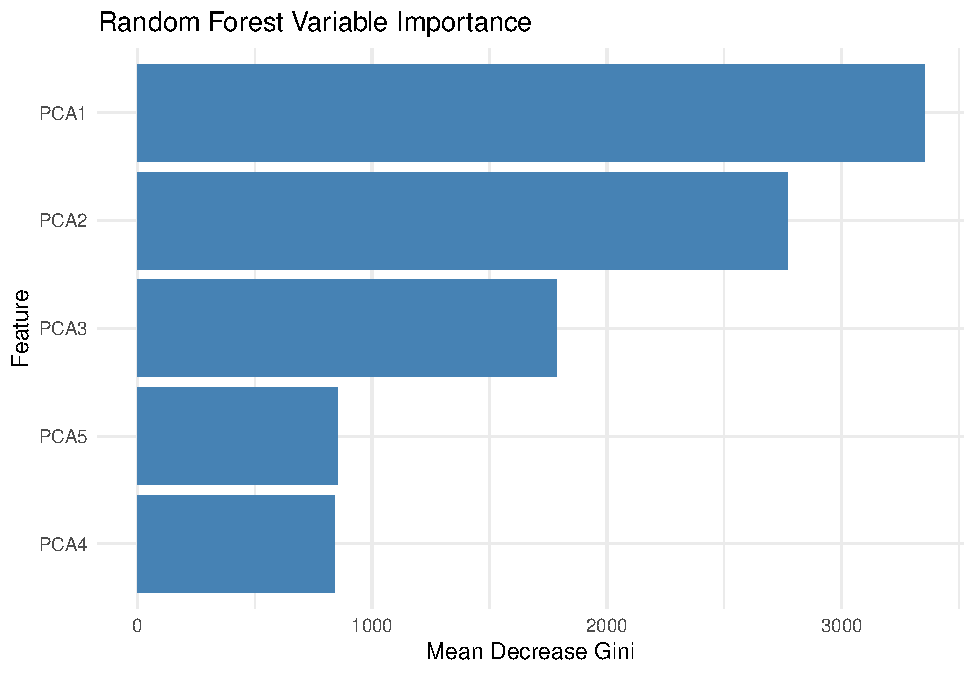
\includegraphics{veg_model_files/figure-latex/unnamed-chunk-17-3.pdf}

\end{document}
